\documentclass[twocolumn]{aastex631}
\bibliographystyle{aasjournal}

\usepackage{graphicx}
\usepackage[caption=false]{subfig}
\usepackage{amsmath}
\usepackage{booktabs}
\usepackage{censor}

\let\pwiflocal=\iffalse \let\pwifjournal=\iffalse
%From: http://arxiv.org/format/1512.00483

\newcommand{\hatp}{\object{HAT-P-67}}
\newcommand{\hatpb}{\object{HAT-P-67 b}}

%% General
\newcommand{\msini}{\ensuremath{m \sin i}}
\newcommand{\mplsini}{\ensuremath{\mpl\sin i}}
\newcommand{\teff}{\ensuremath{T_{\rm eff}}}
\newcommand{\logg}{\ensuremath{\log{g}}}
\newcommand{\vsini}{\ensuremath{v \sin{I_\star}}}
\newcommand{\feh}{\ensuremath{\rm [Fe/H]}}
\newcommand{\logl}{\ensuremath{\log{L}}}
\newcommand{\vmac}{\ensuremath{v_{\rm mac}}}
\newcommand{\vmic}{\ensuremath{v_{\rm mic}}}
% Activity index R'_HK
\newcommand{\rhk}{\ensuremath{R^{\prime}_{HK}}}
% log of R'_HK
\newcommand{\logrhk}{\ensuremath{\log\rhk}}
% S average value
\newcommand{\Savg}{\ensuremath{\langle S\rangle}}


%% ---------------------------------------------------------------------
%% Solar quantities 
\newcommand{\rsun}{\ensuremath{R_\sun}}
\newcommand{\msun}{\ensuremath{M_\sun}}
\newcommand{\lsun}{\ensuremath{L_\sun}}
\newcommand{\loglsun}{\ensuremath{\log{L_\sun}}}
\newcommand{\teffsun}{\ensuremath{T_{eff,\sun}}}
\newcommand{\rhosun}{\ensuremath{\rho_\sun}}
\newcommand{\loggsun}{\ensuremath{\log{g_{\sun}}}}

%% ---------------------------------------------------------------------
%% Stellar quantities 
\newcommand{\rstar}{\ensuremath{R_\star}}
\newcommand{\mstar}{\ensuremath{M_\star}}
\newcommand{\lstar}{\ensuremath{L_\star}}
\newcommand{\astar}{\ensuremath{a_\star}}
\newcommand{\loglstar}{\ensuremath{\log{L_\star}}}
\newcommand{\teffstar}{\ensuremath{T_{\rm eff\star}}}
\newcommand{\rhostar}{\ensuremath{\rho_\star}}
\newcommand{\loggstar}{\ensuremath{\log{g_{\star}}}}

%% ---------------------------------------------------------------------
%% Earth
\newcommand{\rearth}{\ensuremath{R_\earth}}
\newcommand{\mearth}{\ensuremath{M_\earth}}
\newcommand{\learth}{\ensuremath{L_\earth}}
\newcommand{\teffearth}{\ensuremath{T_{\rm eff,\earth}}}
\newcommand{\rhoearth}{\ensuremath{\rho_\earth}}

%% ---------------------------------------------------------------------
%% Planetary
\newcommand{\rpl}{\ensuremath{R_{p}}}
\newcommand{\mpl}{\ensuremath{M_{p}}}
\newcommand{\lpl}{\ensuremath{L_{p}}}
\newcommand{\teffpl}{\ensuremath{T_{\rm eff,{p}}}}
\newcommand{\rhopl}{\ensuremath{\rho_{p}}}
\newcommand{\ipl}{\ensuremath{i_{p}}}
\newcommand{\epl}{\ensuremath{e_{p}}}
\newcommand{\gpl}{\ensuremath{g_{p}}}
\newcommand{\loggpl}{\ensuremath{\log g_{p}}}

\newcommand{\arstar}{\ensuremath{a/\rstar}}
\newcommand{\zrstar}{\ensuremath{\zeta/\rstar}}

%% ---------------------------------------------------------------------
%% Jupiter
\newcommand{\rjup}{\ensuremath{R_{\rm J}}}
\newcommand{\mjup}{\ensuremath{M_{\rm J}}}
\newcommand{\ljup}{\ensuremath{L_{\rm J}}}
\newcommand{\rhojup}{\ensuremath{\rho_{\rm J}}}
\newcommand{\gjup}{\ensuremath{\g_{\rm J}}}

\newcommand{\rjuplong}{\ensuremath{R_{\rm Jup}}}
\newcommand{\mjuplong}{\ensuremath{M_{\rm Jup}}}
\newcommand{\ljuplong}{\ensuremath{L_{\rm Jup}}}
\newcommand{\teffjuplong}{\ensuremath{T_{eff,{\rm Jup}}}}
\newcommand{\rhojuplong}{\ensuremath{\rho_{\rm Jup}}}
\newcommand{\gjuplong}{\ensuremath{\g_{\rm Jup}}}

\providecommand{\eprint}[1]{\href{http://arxiv.org/abs/#1}{#1}}
\providecommand{\adsurl}[1]{\href{#1}{ADS}}
\newcommand{\project}[1]{\textsl{#1}}

%% ---------------------------------------------------------------------
%% Affiliations
\newcommand{\PSUAA}{Department of Astronomy \& Astrophysics, 525 Davey Laboratory, The Pennsylvania State University, University Park, PA, 16802, USA}
\newcommand{\PSUCEHW}{Center for Exoplanets and Habitable Worlds, 525 Davey Laboratory, The Pennsylvania State University, University Park, PA, 16802, USA}
\newcommand{\Princeton}{Department of Astrophysical Sciences, Princeton University, 4 Ivy Lane, Princeton, NJ 08540, USA}
\newcommand{\RUSSELL}{Henry Norris Russell Fellow}
\newcommand{\CFA}{Center for Astrophysics $\vert$ Harvard $\&$ Smithsonian, 60 Garden Street, MS-16, Cambridge, MA 02138, USA}
\newcommand{\UTAustin}{Department of Astronomy, The University of Texas at Austin, 2515 Speedway, Austin, TX 78712, USA}
\newcommand{\MCDonald}{McDonald Observatory and Department of Astronomy, The University of Texas at Austin, 2515 Speedway, Austin, TX 78712, USA}
\newcommand{\UTSpace}{Center for Planetary Systems Habitability, The University of Texas at Austin, 2515 Speedway, Austin, TX 78712, USA}
\newcommand{\Amsterdam}{Anton Pannekoek Institute for Astronomy, University of Amsterdam, Science Park 904, NL-1098 XH Amsterdam, The Netherlands}
\newcommand{\UCSC}{Department of Astronomy \& Astrophysics, University of California, Santa Cruz, 1156 High St, Santa Cruz, CA 95064, USA}
% -------------------------------------------------------

\begin{document}
\shorttitle{HPF spectral analysis}
\shortauthors{TBD}

\title{A large leading tail of atmospheric escape in the HAT-P-67 b system}

\author[0000-0002-4020-3457]{Michael Gully-Santiago}
\affil{\UTAustin}

\author[0000-0003-2649-2288]{Brendan P. Bowler}
\affiliation{\UTAustin}

\author[0000-0001-9662-3496]{William D. Cochran}
\affil{\MCDonald}
\affil{\UTSpace}

\author[0000-0002-1846-196X]{Aishwarya Ganesh}
\affil{\UTAustin}

\author[0000-0001-9811-568X]{Adam L. Kraus}
\affil{\UTAustin}

\author[0000-0001-9626-0613]{Daniel M. Krolikowski}
\affil{\UTAustin}

\author[0000-0003-2152-9248]{Jessica Luna}
\affil{\UTAustin}

\author[0000-0002-1417-8024]{Morgan MacLeod}
\affiliation{\CFA}

\author[0000-0001-9596-7983]{Suvrath Mahadevan}
\affil{\PSUAA}
\affil{\PSUCEHW}

\author[0000-0002-4404-0456]{Caroline V. Morley}
\affil{\UTAustin}

\author[0000-0001-8720-5612]{Joe P.\ Ninan}
\affil{\PSUAA}
\affil{\PSUCEHW}

\author[0000-0002-9584-6476]{Antonija Oklop{\v{c}}i{\'c}}
\affil{\Amsterdam}

\author[0000-0001-7409-5688]{Guðmundur Stefánsson}
\affil{\Princeton}
\affil{\RUSSELL}

\author[0000-0001-6532-6755]{Quang H. Tran}
\affiliation{\UTAustin}

\author[0000-0002-3726-4881]{Zhoujian Zhang}\thanks{NASA Sagan Fellow}
\affiliation{\UCSC}

% and more...

\collaboration{1}{HPF Helium Exospheres Collaboration}

\begin{abstract}
    To be overhauled...
\end{abstract}

\keywords{stars: fundamental parameters ---  stars: statistics}

\section{Introduction}\label{sec:intro}

Atmospheric escape appears to be a compulsory phase for exoplanets of a certain size and insolation, statistically imprinted in the dearth of 1.5-2.0~$R_\oplus$ planets \citep{2017AJ....154..109F}.  The two physical mechanisms for this rapid transition between mini-Neptunes and super-Earths include photoevaporation \citep{2013ApJ...775..105O,2017ApJ...847...29O} and core-powered mass loss \citep{2019MNRAS.487...24G}.  Whatever the cause, some large fraction of planets must undergo atmospheric escape and the signal should be widely discernable, at least in observationally favorable configurations such as transiting planets.

Enough uncertainty exists in the tradeoffs among physical mechanisms, system ages, and timescales to make it unclear whether any given exoplanet will be actively undergoing atmospheric escape.  The most favorable traits may include close-in, low surface gravity exoplanets within a strategically chosen radius range.  The 1.5-2.0 Earth radius range could be expected to harbor atmospheres that have not yet shed their gaseous envelopes, still in the act of descending to their final state.  Alternatively, inflated Hot Jupiters could be so dramatically ablated as to overcome the somewhat stronger potential well.  Significant gains in understanding can therefore be expected from observational studies sampling the extremes of the exoplanet distribution.

Candidates for detection should be observable in one of three atomic lines.  Ly~$\alpha$, \ion{He}{1} 10833 \AA, and H~$\alpha$ have emerged as the most amenable to detection \citep{2018ApJ...855L..11O,2023MNRAS.518.4357O}.  Ly $\alpha$ can exhibit strong atmospheric escape signals, but instellar medium \ion{H}{1} absorption censors its low-velocity linecore.  \ion{He}{1} 10833 \AA~ offers significant advantages over Ly~$\alpha$, and has resulted in 8 systems with detections to date: \object[GJ 3470]{GJ3470} \citep{2020ApJ...894...97N, 2021A&A...647A.129L}, \object{HD 63433 c} \citep{2022AJ....163...68Z}, WASP 107 b \citep{2019A&A...623A..58A,2020AJ....159..115K}, HD 209458 b \citep{2019A&A...629A.110A}, WASP 69 b \citep{2020AJ....159..278V}, WASP 52 b \citep{2020AJ....159..278V}, HD 189733 b \citep{2021A&A...647A.129L}, and HAT-P-18 b \citep{2021ApJ...909L..10P}.  These detections exhibit a range of signal strengths, as high as 10$\%$ transit depths.  Measurements at high spectral resolution have been especially valuable for evincing velocity substructure of the escaping gas motion relative to the exoplanet restframe \citep{2019A&A...629A.110A,2020ApJ...894...97N}, and convincingly associating the signal to an exoplanetary origin as opposed to stellar contamination \citep{2018AJ....156..189C}.


Here we present a study of the exosphere of \object{HAT-P-67 b}, an inflated hot Saturn orbiting an F type sub-giant\footnote{The system appears to consist of a binary with an M dwarf companion HAT-P-67B separated on-sky by $9\farcs0$ \citep{2019MNRAS.490.5088M}.  The IAU naming convention would demand HAT-P-67Ab.  We simply drop the A designation for notational simplicity, since the wide companion will not factor into our analysis.} at a distance of 0.06 AU \citep{2017AJ....153..211Z}.  The strong insolation combined with \object{HAT-P-67 b}'s low surface gravity makes it an excellent candidate for strong atmospheric mass loss.  It orbits an evolved star, opening the prospect for the planet's insolation to have increased over time as the star grew.  These and other reasons make \object{HAT-P-67 b} a predestined laboratory for measuring the properties of exospheres at the extreme.


\section{Observations}
\subsection{Habitable Zone Planet Finder (HPF)}

The Habitable Zone Planet Finder Spectrograph \citep[HPF;][]{2012SPIE.8446E..1SM,2014SPIE.9147E..1GM, 2019Optic...6..233M} on the queue-scheduled 10-meter \emph{Hobby-Eberly Telescope} \citep[HET;][]{1998SPIE.3352...34R} operates in the near-IR from $8100-12800~$\AA~ spanning the \textit{z}, \textit{Y}, and \textit{J} bands at spectral resolving power $R=55,000$. The HET fixed-elevation design \citep{2007PASP..119..556S} limits the observability of \object{HAT-P-67} to less than 1 hour ``tracks'' for a fixed range of hour angles before (east track) and after (west track) the star transits the meridian.  Whereas conventional steerable telescopes could conduct continuous point-and-stare observations of \object{HAT-P-67} for hours, HET cannot.  In practice, this limitation means that in-transit and out-of-transit observational phases were rarely possible on the same night.  Instead, we organized the observations into four campaigns to coincide with \object{HAT-P-67 b} transits on the nights beginning 2020 April 28, 2020 May 22, 2020 June 15, and 2022 April 28.  These in-transit nights had up to 14 exposures per HET track, with integration times between 5-8.5 minutes.  We obtained out-of-transit baseline observations up to 2 nights before and after the transit, plus random-in-phase low priority P4 queue-filler observations.  These out-of-transit observations typically received 4 or fewer individual exposures.  We observed HAT-P-67 with HPF for a total 41 visits on 39 unique nights, with two of those nights observing both an east and a west track.  The total on-source integration time exceeds 13.8 hours.  Table \ref{tabHPFLog} summarizes the log of observations.

The observation scheduling was strategically restricted to the spring season when the Barycentric Earth Radial Velocity (BERV) would Doppler shift telluric absorption lines sufficiently far away from the core of the Helium 10833$\AA~$ feature.  The small BERV still means the redward Helium linewing has significant telluric contamination between 10834-10836 \AA, but the core and blue line wings appear relatively pristine.

Only 19 out of the 39 nights possess A0V telluric calibration standard stars.  These standard stars, when available, were used to spot-check our telluric mitigation strategy.


\begin{deluxetable}{lccrchr}
    \tablewidth{0pc}
    \tabletypesize{\scriptsize}
    \tablecaption{
        HPF Observation Log
        \label{tabHPFLog}
    }
    \tablehead{
        \colhead{Date}   &
        \colhead{Track} &
        \colhead{Transit?} &
        \colhead{BTJD} &
        \colhead{$N_\mathrm{exp}$} &
        \nocolhead{$t_\mathrm{exp}$} &
        \colhead{$\phi$}\\
        \colhead{}   &
        \colhead{} &
        \colhead{} &
        \colhead{(days)} &
        \colhead{} &
        \nocolhead{(s)} &
        \colhead{$\in(-0.5, 0.5)$}
    }
    \startdata
    2020-04-26 &  east &                 & 1966.78 &             4 & 308.85 &            -0.192 \\
2020-04-27 &  east &      in transit & 1967.79 &            12 & 308.85 &             0.018 \\
2020-04-28 &  east &                 & 1968.78 &             4 & 308.85 &             0.225 \\
2020-05-19 &  west &                 & 1989.95 &             4 & 308.85 &            -0.373 \\
2020-05-20 &  west &                 & 1990.94 &             4 & 308.85 &            -0.169 \\
2020-05-21 &  east &      in transit & 1991.72 &            14 & 308.85 &            -0.006 \\
2020-05-22 &  west &                 & 1992.93 &             4 & 308.85 &             0.246 \\
2020-05-23 &  west &                 & 1993.94 &             4 & 308.85 &             0.455 \\
2020-06-12 &  west &                 & 2013.89 &             3 & 308.85 &            -0.397 \\
2020-06-13 &  west &                 & 2014.89 &             4 & 308.85 &            -0.190 \\
2020-06-14 &  east &                 & 2015.64 &             6 & 308.85 &            -0.032 \\
2020-06-14 &  east &      in transit & 2015.66 &             3 & 308.85 &            -0.029 \\
2020-06-14 &  west &      in transit & 2015.89 &             9 & 308.85 &             0.019 \\
2020-06-15 &  west &                 & 2016.87 &             4 & 308.85 &             0.224 \\
2020-06-17 &  west &                 & 2018.88 &             4 & 308.85 &            -0.360 \\
2020-07-21 &  west &                 & 2052.79 &             2 & 511.20 &            -0.309 \\
2020-07-31 &  west &                 & 2062.75 &             2 & 511.20 &            -0.240 \\
2021-01-30 &  east &                 & 2246.03 &             2 & 511.20 &            -0.136 \\
2021-01-31 &  east &                 & 2247.02 &             2 & 511.20 &             0.070 \\
2021-02-23 &  east &                 & 2269.96 &             1 & 511.20 &            -0.161 \\
2021-02-25 &  east &                 & 2271.94 &             2 & 511.20 &             0.250 \\
2021-03-03 &  east &                 & 2277.93 &             2 & 511.20 &             0.496 \\
2021-03-30 &  east &                 & 2304.86 &             2 & 511.20 &             0.094 \\
2022-04-27 &  east &                 & 2697.79 &             4 & 308.85 &            -0.217 \\
2022-04-28 &  east &      in transit & 2698.78 &            14 & 308.85 &            -0.011 \\
2022-04-29 &  east &                 & 2699.77 &             4 & 308.85 &             0.196 \\
2022-04-30 &  east &                 & 2700.77 &             4 & 308.85 &             0.403 \\
2022-05-01 &  east &                 & 2701.77 &             4 & 308.85 &            -0.390 \\
2022-06-19 &  east &                 & 2750.64 &             3 & 308.85 &            -0.230 \\
2022-06-21 &  east &                 & 2752.64 &             3 & 308.85 &             0.187 \\
2022-06-21 &  west &                 & 2752.86 &             3 & 308.85 &             0.232 \\
2022-06-22 &  west &                 & 2753.86 &             3 & 308.85 &             0.439 \\
2022-06-25 &  east &      in transit & 2756.64 &             1 & 308.85 &             0.017 \\
2022-06-30 &  west &                 & 2761.85 &             1 & 308.85 &             0.101 \\
2022-07-09 &  west &                 & 2770.82 &             1 & 308.85 &            -0.035 \\
2022-07-10 &  west &                 & 2771.81 &             1 & 308.85 &             0.172 \\
2022-07-12 &  west &                 & 2773.82 &             3 & 308.85 &            -0.411 \\
2022-07-14 &  west &      in transit & 2775.78 &             1 & 308.85 &            -0.003 \\
2022-07-15 &  west &                 & 2776.80 &             1 & 308.85 &             0.209 \\
2022-07-19 &  west &                 & 2780.77 &             1 & 308.85 &             0.034 \\
2022-07-28 &  west &                 & 2789.74 &             1 & 308.85 &            -0.101 \\
2022-07-29 &  west &                 & 2790.78 &             1 & 308.85 &             0.115 \\
    \enddata
    \tablecomments{All exposure times were 308.85~s except for observations from 2020-07-21 to 2021-03-30, which were 511.20~s.}
\end{deluxetable}

\subsection{TESS Light Curves}
HAT-P-67 was observed with the \emph{Transiting Exoplanet Survey Satellite} \citep[TESS,][]{2014SPIE.9143E..20R} in Sectors 24, 26, 51, 52, 53 with 2-minute cadence, and in Sector 25 with 30-minute (FFI) cadence.  The Sector 25 FFI data appeared malformed, possibly due to problems with pipeline CCD smear correction, and was disregarded.

We also assembled a comparison sample of about 1000 lightcurves to interpret the  prevalence of lightcurve modulation and stellar activity among broadly F subgiant-like stars.  We selected sources based on \emph{Gaia} DR3 $T_\mathrm{eff}$ estimates and similar $\log{g}$,  and availability of at least one sector of TESS 2-minute cadence data\footnote{The requirement to have 2-minute cadence data---a data reduction convenience---may include biases stemming from the pre-selection of TESS targets, but it is not clear whether such a pre-selection would favor more or less stellar activity}.  We also visually spot-checked these lightcurves to understand artifacts and windowing effects.

\subsection{ASAS-SN}
We retrieved ground-based photometry with the \emph{All-Sky Automated Survey for Supernovae} (ASAS-SN) using the Sky-Portal \citep{shappee14,2017PASP..129j4502K}.  The precision of ASAS-SN was too low to perceive stellar variability, and so the photometry is not presented further.

\subsection{DASCH}
HAT-P-67 appears in the Harvard Plate Archive, with 5809 measurements digitized through DASCH, spanning over 120 years of coarse photometric monitoring.  In principle these datasets could inform long-term variability trends such as stellar cycles.  In practice the 0.15 magnitude jitter appears too coarse to perceive any genuine astrophysical variability, with no conspicuous trend seen.  We can therefore place a relatively mild constraint that the star is stable at the $30\%$ level over periods of tens to hundreds of years.

\subsection{Gaia DR3}
HAT-P-67A (\emph{Gaia DR3 1358614983131339392}) has a parallax of $2.69\pm0.01$ mas in \emph{Gaia} DR3, placing it at about 372$\pm$1.4 pc, slightly farther than previously estimated by \citet{2017AJ....153..211Z} using Gaia DR1. Its coarse Gaia-based estimates for RV and Doppler broadening are consistent with the more precise values published in \citet{2017AJ....153..211Z}.  Its wide companion HAT-P-67B (\emph{Gaia DR3 1358614983131339904}) \citep{2019MNRAS.490.5088M} has statistically identical parallax ($2.58\pm0.05$) and proper motions, confirming its interpretation as co-moving, with projected separation of about 3400 AU.

\subsection{Other archives}
We searched for observations of HAT-P-67 in public archives.  It has one $R\sim8000$ spectrum from the Intermediate Dispersion Spectrograph on the INT, centered near 4000 \AA.  It has 26 photometry points from \emph{Pan-STARRS} spread across its 5 filters.  The other archival observations have been previously reported by \citet{2017AJ....153..211Z}, including Keck HIRES, Keck NIRC2, and WIYN High-Resolution Infrared Camera.  The northern source does not appear in ESO archives, nor the Gemini Archive, and it is not publicly accessible in the Zwicky Transient Factory (ZTF) archive.  It was not targeted by \emph{Spitzer} or \emph{Hubble}.

\begin{figure*}
    \centering
    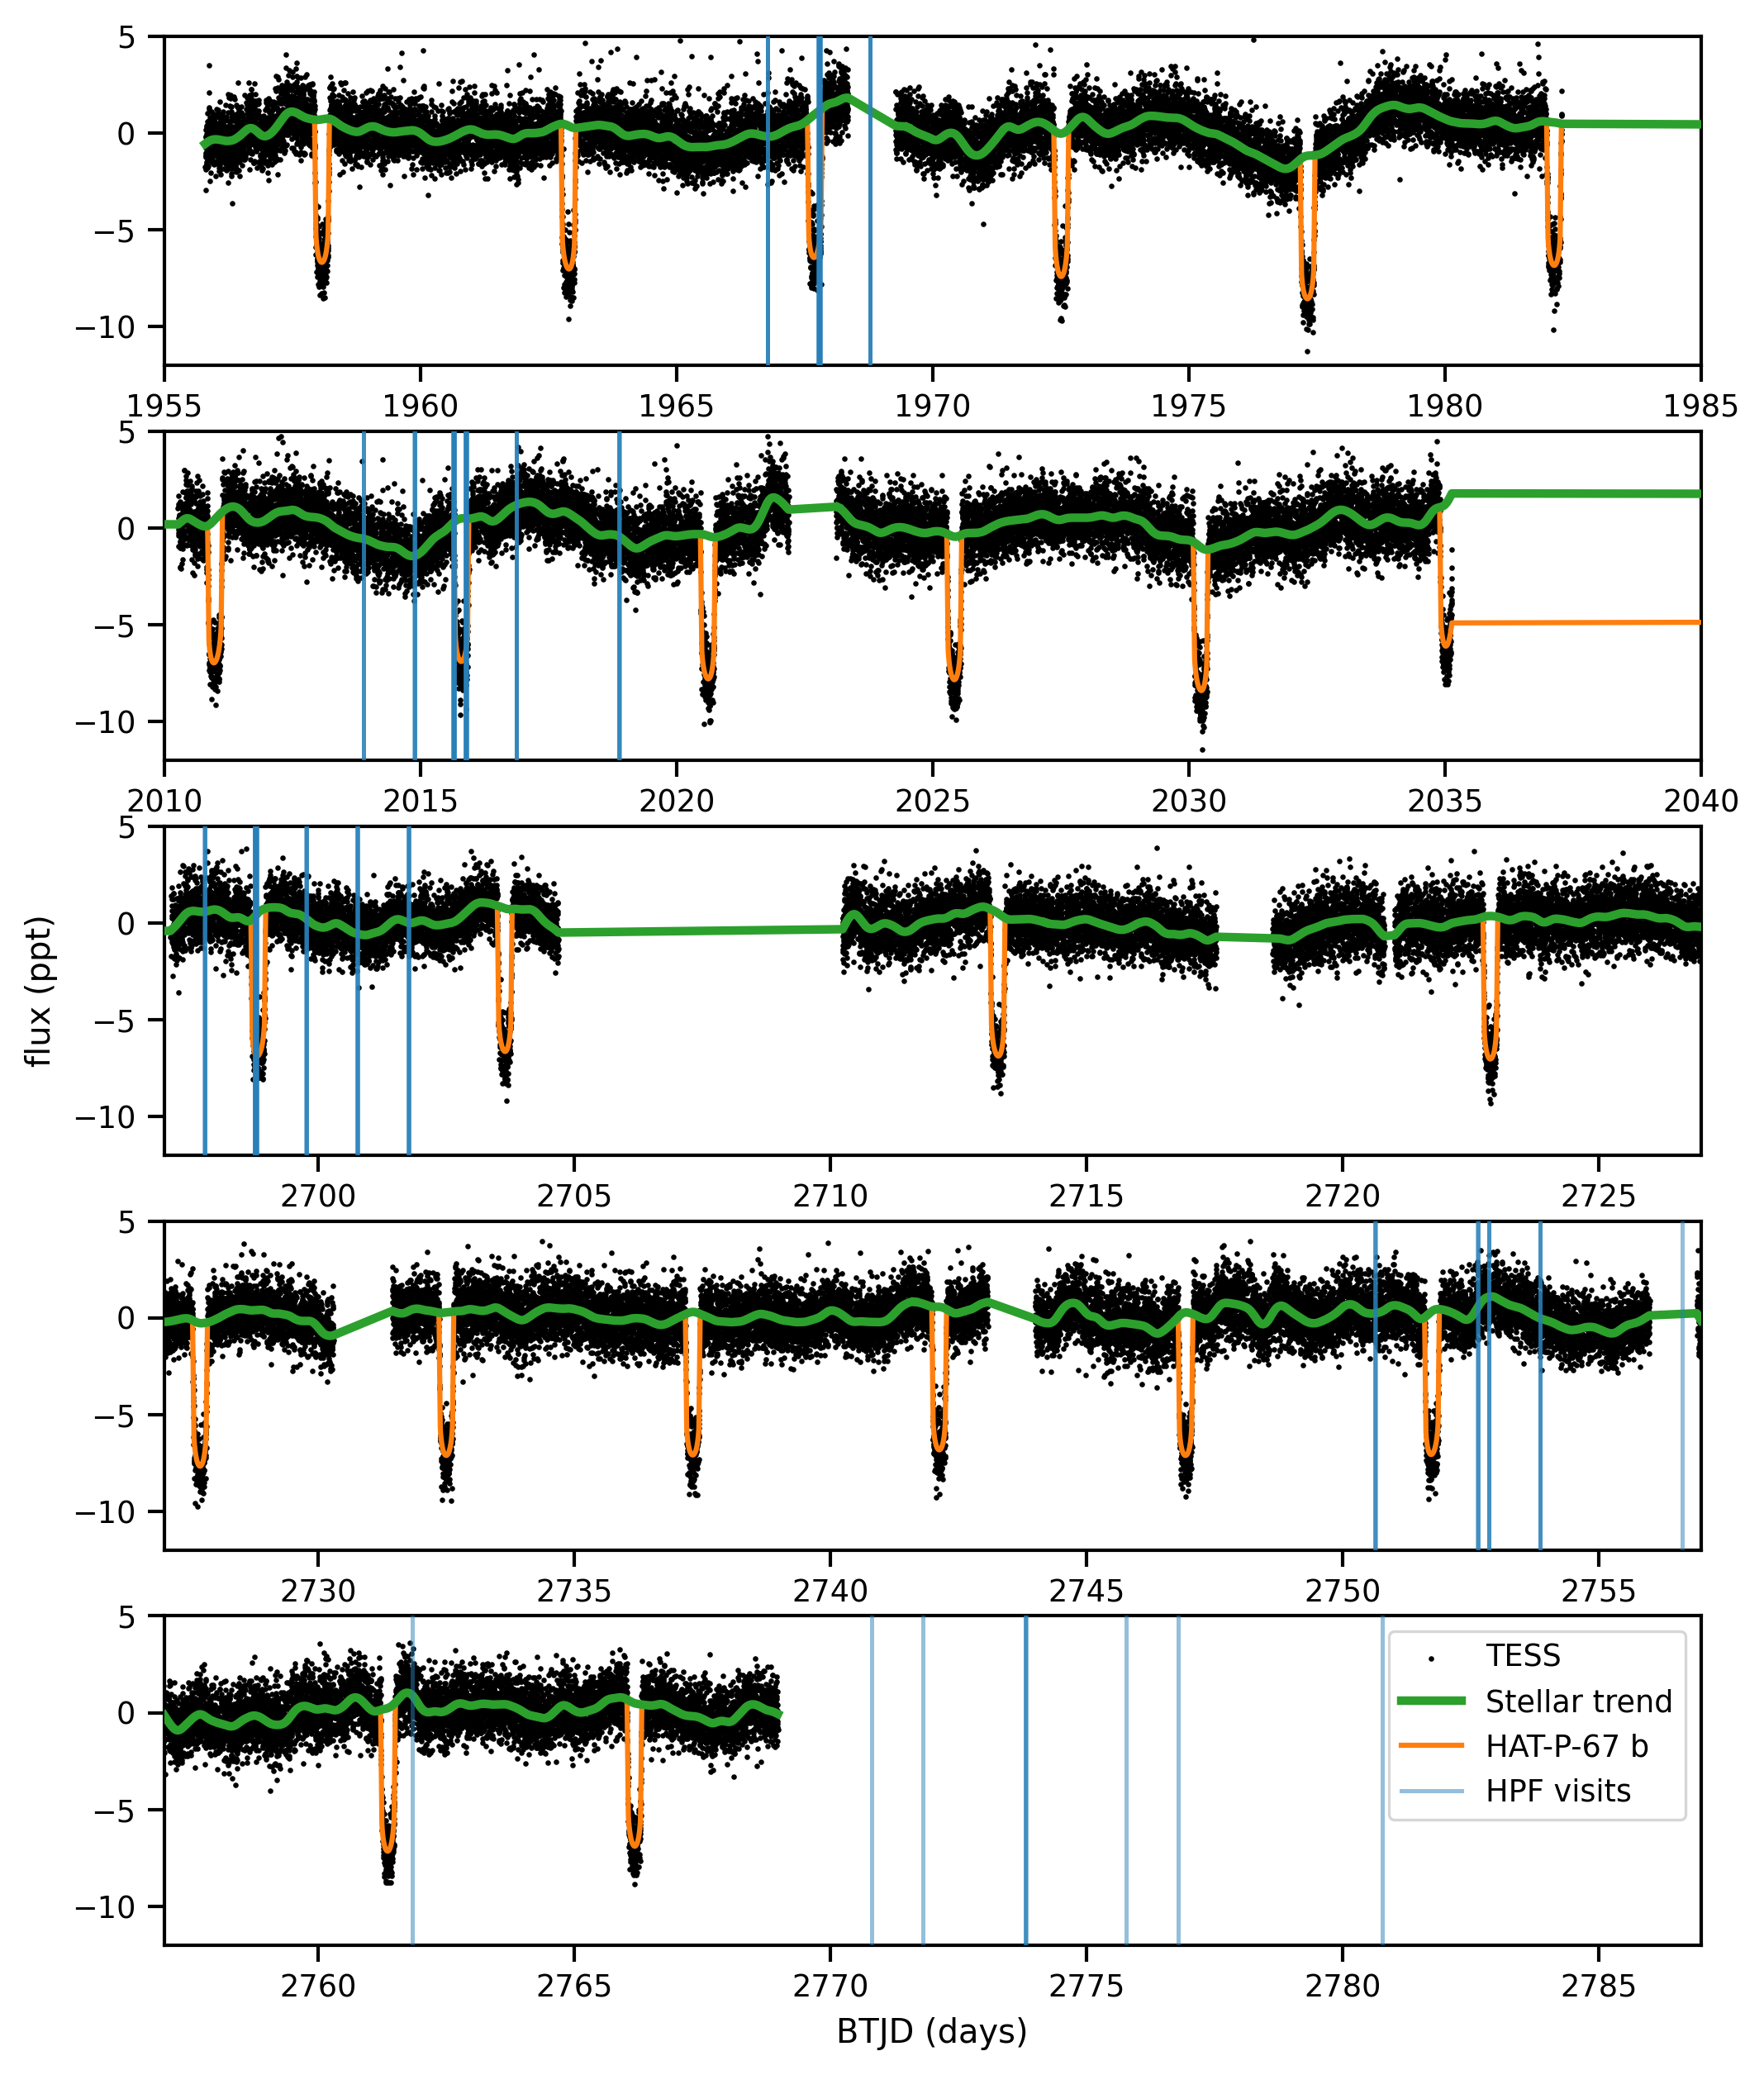
\includegraphics[width=0.7\linewidth]{figures/TESS_HAT-P-67b_overview.png}
    \caption{Overview of all available TESS Sectors showing 24 full or partial transits with 34 visits with HPF (vertical gray bars), 7 of which coincide with transits, and the rest sample out-of-transit phase.  The 8 HPF visits between BTJD 2050 and 2690 are not shown.}
    \label{fig:TESSoverview}
\end{figure*}


\section{Analysis}

\subsection{TESS Light Curve}
Previously, \hatp transits had only been detected with \emph{HATNet} \citep{2004PASP..116..266B} and followed up with KeplerCam on the FLWO 1.2 m telescope. These ground-based photometers were not intended to measure, and did not detect, long term stellar variability signals.  We therefore examined the \emph{TESS} lightcurves for out-of-transit photometric variability.
\subsubsection{Revised exoplanet orbital parameters}
We assembled a composite lightcurve by stitching TESS Sectors 24, 26, 51, 52, 53, which were reduced with the default SPOC pipeline \citep{2020RNAAS...4..201C}, and lightly post-processed with \texttt{lightkurve} \citep{geert_barentsen_2019_2565212}.  These TESS data exhibit an RMS scatter of better than 1 part-per-thousand (ppt) at native 2-minute sampling.  We fit a Keplerian orbit model to the TESS lightcurve using the \texttt{exoplanet} framework \citep{exoplanet:joss}.  We obtained a best fit orbital period of $4.81011$ days, non-zero eccentricity of 0.19, an impact parameter of 0.46, planet-to-star radius ratio of 0.0823, transit depth of 0.74\%, and $T_0$ of 1958.07933 in BTJD.  These properties are consistent with the previously reported values from \citet{2017AJ....153..211Z} and the updated ephemeris of \citet{2022ApJS..259...62I}.  Figure \ref{fig:TESSoverview} shows an overview of all the TESS Sectors demarcated with the epochs of HPF measurements.  Figure \ref{fig:transit} shows the best-fit orbit overlaid on the detrended TESS lightcurve.  Table \ref{tabOrbit} lists one of the previous orbit determinations and solution reported here.



\subsubsection{Stellar rotation rate from periodogram analysis}

The TESS Sector 26 lightcurve exhibits a weak $\sim3\;$ppt peak-to-valley out-of-transit modulation on timescales comparable to the exoplanet orbit. TESS Sectors 51-53 do not show as conspicuous a modulation signal.  Figure \ref{fig:TESSmodulation} shows this modulation in the minimally processed TESS lightcurve.  During the exoplanet orbit fitting, we fit the TESS lightcurve modulation with a quasiperiodic Gaussian Process (GP) model using \texttt{celerite} \citep{celerite1,celerite2}.  The GP model fit to the entire composite lightcurve yields a period of 4.7 days; when fit to individual sectors alone the periods hover around 5.9 days.

If we attribute the TESS modulation signal to stellar activity, we obtain a rotation period $P_\mathrm{rot}$ between 4.7 and 5.9 days.  \citet{2017AJ....153..211Z} estimated $v\sin{i}=35.8\pm1.1$ km/s, or lower ($v\sin{i}=30\pm1.1$ km/s) if macroturbulence was accounted for.  Assuming a stellar radius of 2.1-2.7 $R_\odot$, we obtain combined geometric constraint $3.0 < \frac{P_\mathrm{rot}}{\sin{i}}  < 4.5 $ days.  This range is close to---but slightly lower than---the TESS modulation period.   The Gaia \emph{DR3}-derived distance is 8\% greater than the \emph{Gaia} DR1 estimate used in \citet{2017AJ....153..211Z}; the revised larger distance would tend to increase the radius estimate by 16\% to match the observed SED in isochrone-fitting.  We would therefore expect an isochrone-derived $R_\star$ range closer to $2.5-3.14 R_\odot$, where we have dropped the 1-$\sigma$ uncertainties which had included the less certain Gaia DR 1 parallax and its uncertain correction terms.  For a fixed $R_p/R_\star$, the larger $R_\star$ implies a proportionally larger planet radius, revising the already-low density of HAT-P-67 even lower.

\begin{figure}
    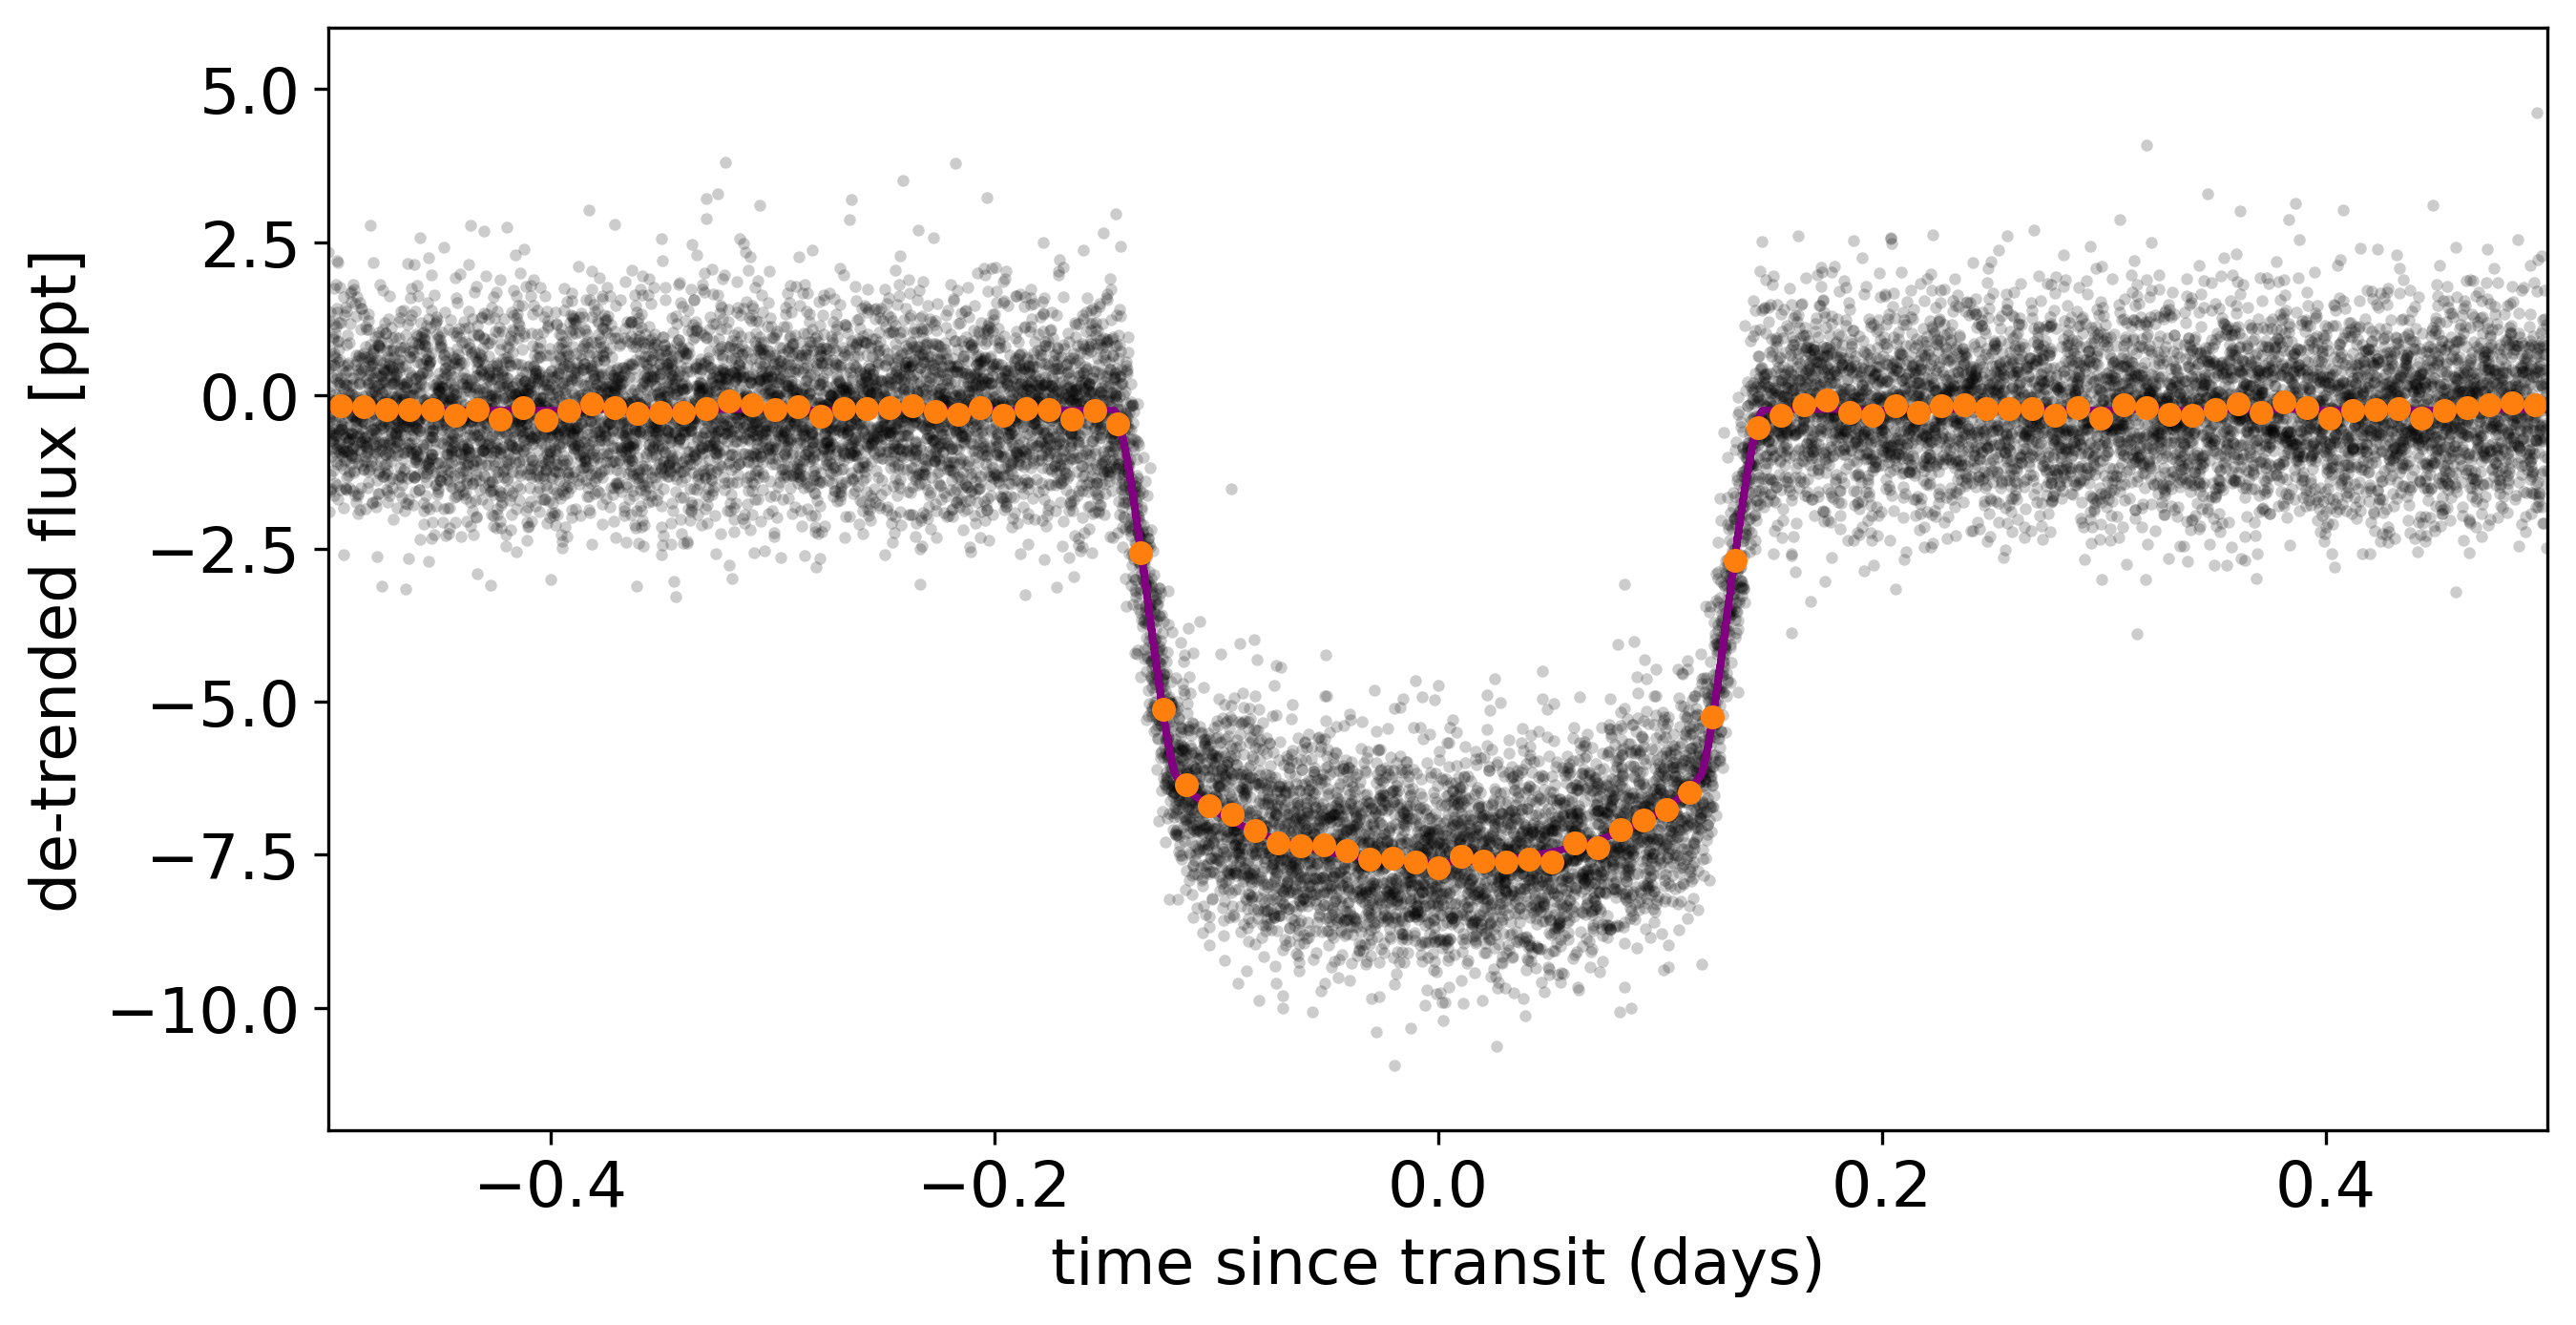
\includegraphics[width=\linewidth]{figures/best_fit_orbit.png}
    \caption{Best fit orbit overlaid on the composite TESS lightcurve.}
    \label{fig:transit}
\end{figure}

\subsubsection{Lightcurve modulation amplitude}
Finally, we computed the peak-to-valley modulation for the 1000-lightcurve comparison sample, defined as the difference between the 90$^{th}$ to 10$^{th}$ percentile of each normalized TESS lightcurve.   We find that most lightcurves are consistent with negligible astrophysical variability and/or variability predominated by instrumental artifacts. Nevertheless, \object{HAT-P-67 b}'s 0.36$\%$ lightcurve modulation was slightly larger than the typical comparison source, ranking in the 87$^{th}$ percentile of the ensemble.  However the higher-modulation sources exhibited 3-5$\times$ the level of modulation seen in \object{HAT-P-67 b}, whereas \object{HAT-P-67 b} was only about 0.5$\times$ above the median.


\begin{deluxetable*}{lrrrh}
    \tablewidth{0pc}
    \tabletypesize{\scriptsize}
    \tablecaption{
        Revised orbital and planetary parameters
        \label{tabOrbit}
    }
    \tablehead{
        \colhead{Parameter}   &
        \colhead{Zhou et al. 2017} &
        \colhead{Ivshina \& Winn 2022} &
        \colhead{This Work} &
        \nocolhead{Alternate}
    }
    \startdata
    %%
    ~~~$P$ (days)             \dotfill    & $4.8101025_{-3.3\times 10^{-7}}^{+4.3\times 10^{-7}}$ & 4.8101046$\pm1.7\times10^{-6}$ & 4.81011 & z \\
    ~~~$T_c$ (${\rm BTJD}$)  \dotfill    & $-1038.61533_{-0.00064}^{+0.00076}$ & 1958.08059$\pm$0.00032 & 1958.07933 & z \\
    ~~~$T_{14}$ (hours)  \dotfill    & $6.9888 \pm 0.046$ &  & 7.0636 & z \\
    ~~~$\rpl/\rstar$          \dotfill    & $0.0834\pm0.0017$ &  & 0.08231 & z \\
    ~~~$b \equiv a \cos i/\rstar$
    \dotfill    & $0.12_{-0.08}^{+0.12}$ &  & 0.45616 & z \\
    \enddata
\end{deluxetable*}


\subsection{HPF analysis}
The raw 2D echellograms were reduced with the \texttt{Goldilocks} package\footnote{\url{https://github.com/grzeimann/Goldilocks_Documentation}}, which outputs 1D extracted spectra for the target, and two reference fibers: blank sky and a laser frequency comb (LFC).  The observations were acquired with the LFC turned off, so this unilluminated spectrum was discarded.

The sky fiber and target fiber have slightly different throughputs and illumination properties so the sky fiber must be scaled prior to subtraction from the target spectrum.  On average the target fiber sees $93\%$ of the flux of the sky reference fiber, and at the few percent level this ratio depends on wavelength and season.  We quantified the wavelength dependence by acquiring calibration observations of blank sky in both the target and sky fiber.  We applied this wavelength-based scale factor to each target spectrum's associated reference sky fiber to achieve near-imperceptible sky-line residuals.  A few lines exhibit residuals which may arise from genuine differences in the local atmospheric conditions between the target and sky fiber.

We masked spectral regions predicted to have significant telluric lines with a template generated by \texttt{telfit} \citep{2014AJ....148...53G}.  We shifted the spectral coordinates to their common barycentric-corrected reference frame \citep{2014PASP..126..838W} as implemented in \texttt{astropy} \citep{2013A&A...558A..33A,2018AJ....156..123A,2022ApJ...935..167A}.  We flattened the spectra to two pre-selected continuum indices highlighted as vertical blue bands in Figure \ref{fig:HPFheliumOverview}.  The sky-subtraction, telluric masking, barycentric correction, flattening, and all of our other standard pre-processing steps were carried out in the open-source Python interface \texttt{muler} \citep{2022JOSS....7.4302G}.

Figure \ref{fig:HPFheliumOverview} shows a zoom-in on the He 10830 region of interest, with all 153 individual exposures overlaid.  We see a variability in the Helium line of up to 10\%, much greater than the $<1\%$ pixel-to-pixel variation.  The feature width spans about 3~\AA, comparable to the stellar rotationally broadened lines and too broad to originate from the much narrower telluric lines.

\begin{figure}
    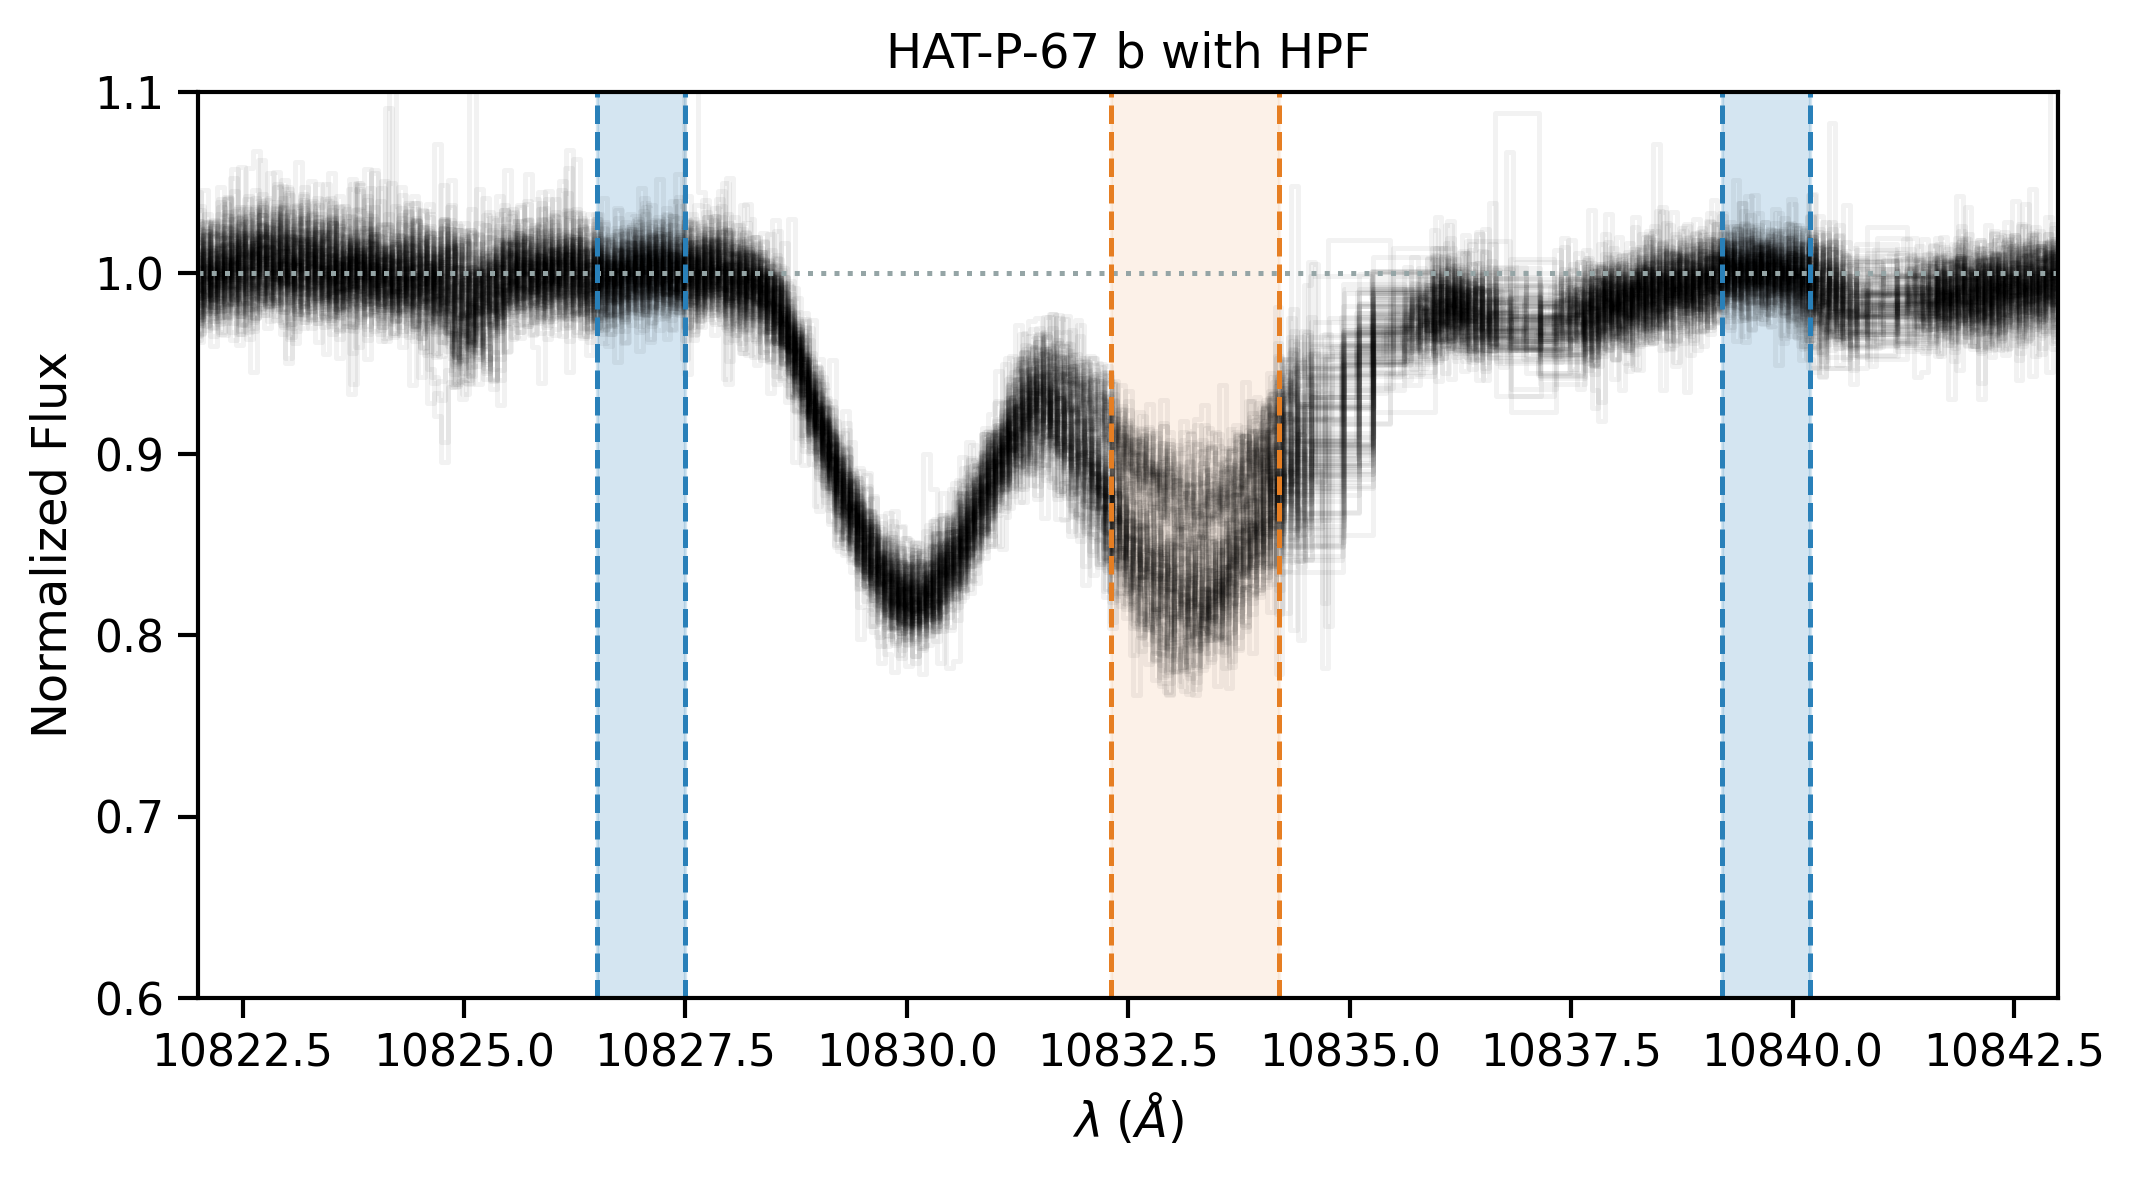
\includegraphics[width=\linewidth]{figures/HAT_P_67b_He_spectrum.png}
    \caption{Overlay of all 128 individual HPF exposures of HAT-P-67, spanning 2020-2022. Variability is seen in the \ion{He}{1} 10833 \AA~ triplet, denoted by the vertical orange shaded band, but not in the adjacent regions.  These snapshot spectra were barycentric corrected, and continuum flattened to the regions in the blue vertical bands.  Sharp telluric absorption lines have been masked in regions near 10835 and 10837.5 $\AA$.}
    \label{fig:HPFheliumOverview}
\end{figure}


The 13.8 hours of exposure, combined with \object{HAT-P-67 b}'s short ($P\sim4.8$ day) period, means that a large fraction of the orbit has been collected, with some phases (especially near transit) heavily sampled, and some other out-of-transit phases sampled only sparsely. We constructed a 2-D intensity phase scan, binning in phase and wavelength, and spanning the entire orbit of \object{HAT-P-67 b}.  Figure \ref{fig:HPFphase2D} overlays the planet's approximately $\pm150\;$km/s orbital Doppler velocity, with the stellar rest frame velocity demarcated by the vertical line.  The vanishing $<36$ m/s reflex motion of the star is imperceptible at this scale.  The horizontal dashed lines indicate the transit ingress, midcenter, and egress.

\begin{figure}
    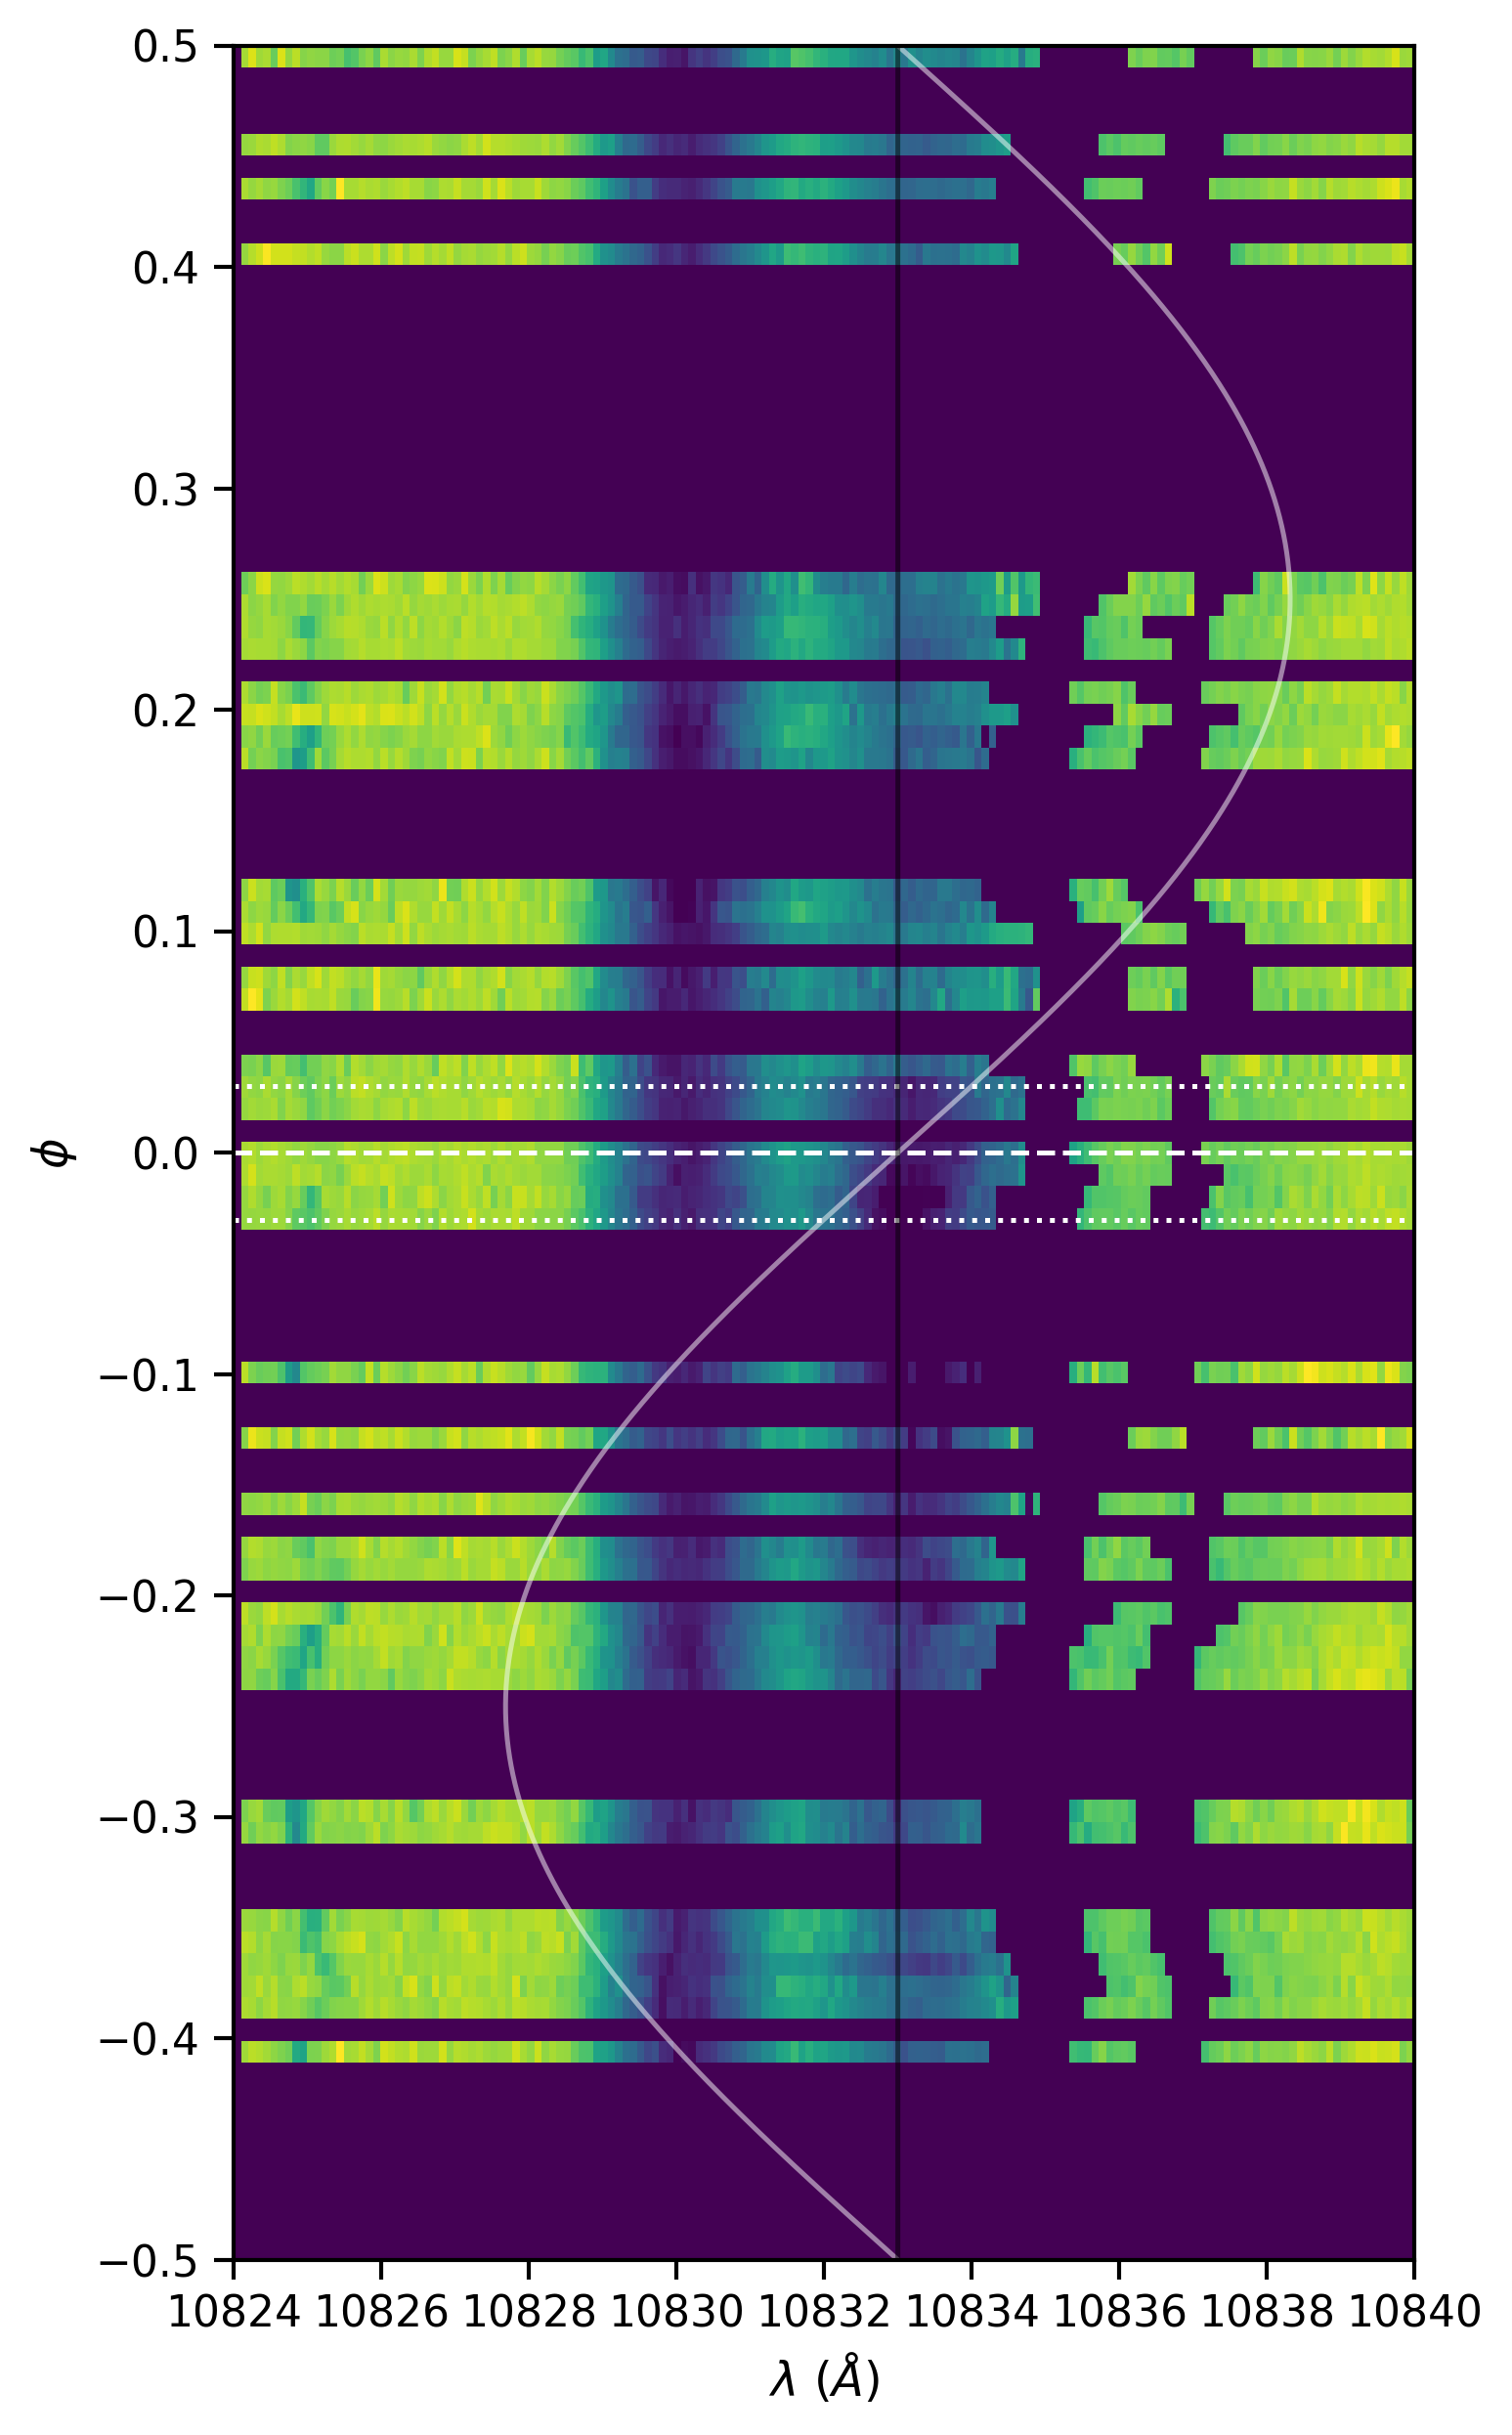
\includegraphics[width=0.8\linewidth]{figures/phase_2D_diagram.png}
    \caption{Phase scan of intensity for HAT-P-67.  The spectrum flux intensity shows significant in-transit absorption during and before the transit.  Telluric lines redward of the line center have been masked.  An unmasked telluric line near 10825 \AA~ can be seen.}
    \label{fig:HPFphase2D}
\end{figure}

A large absorption signal can be seen preceding transit ingress, with some significant absorption evident before $-0.2$ in phase.  We construct a fractional residual absorption spectrum by subtracting off and re-normalizing to the non-varying baseline.  We define the non-varying baseline spectrum as the average over phases $0.3-0.5$, which exhibited stable spectra with the least absorption.  Figure \ref{fig:HPFscanResid} shows a conspicuous view of the Helium absorption of \object{HAT-P-67 b}.  Significant absorption can be seen as a few percent at $-0.37$ in phase, rising to 10\% just before and during transit.  The egress drop off is extremely sharp, with almost no absorption directly after transit.

The absorption resides mostly near the stellar zero restframe velocity reference.  As mentioned previously, the telluric masking near 10836 \AA~ censors our view of the existence (or not) of any redshifted lobe in this region.  A more careful treatment of the telluric absorption could rescue some of the data in this region.

Finally, a tentative much weaker post-egress bifurcation into blue-shifted absorption and redshifted emission may exist near 0.1 in phase.  The signal appears at or just above the noise level, but is shared among tens of pixels.


\begin{figure}
    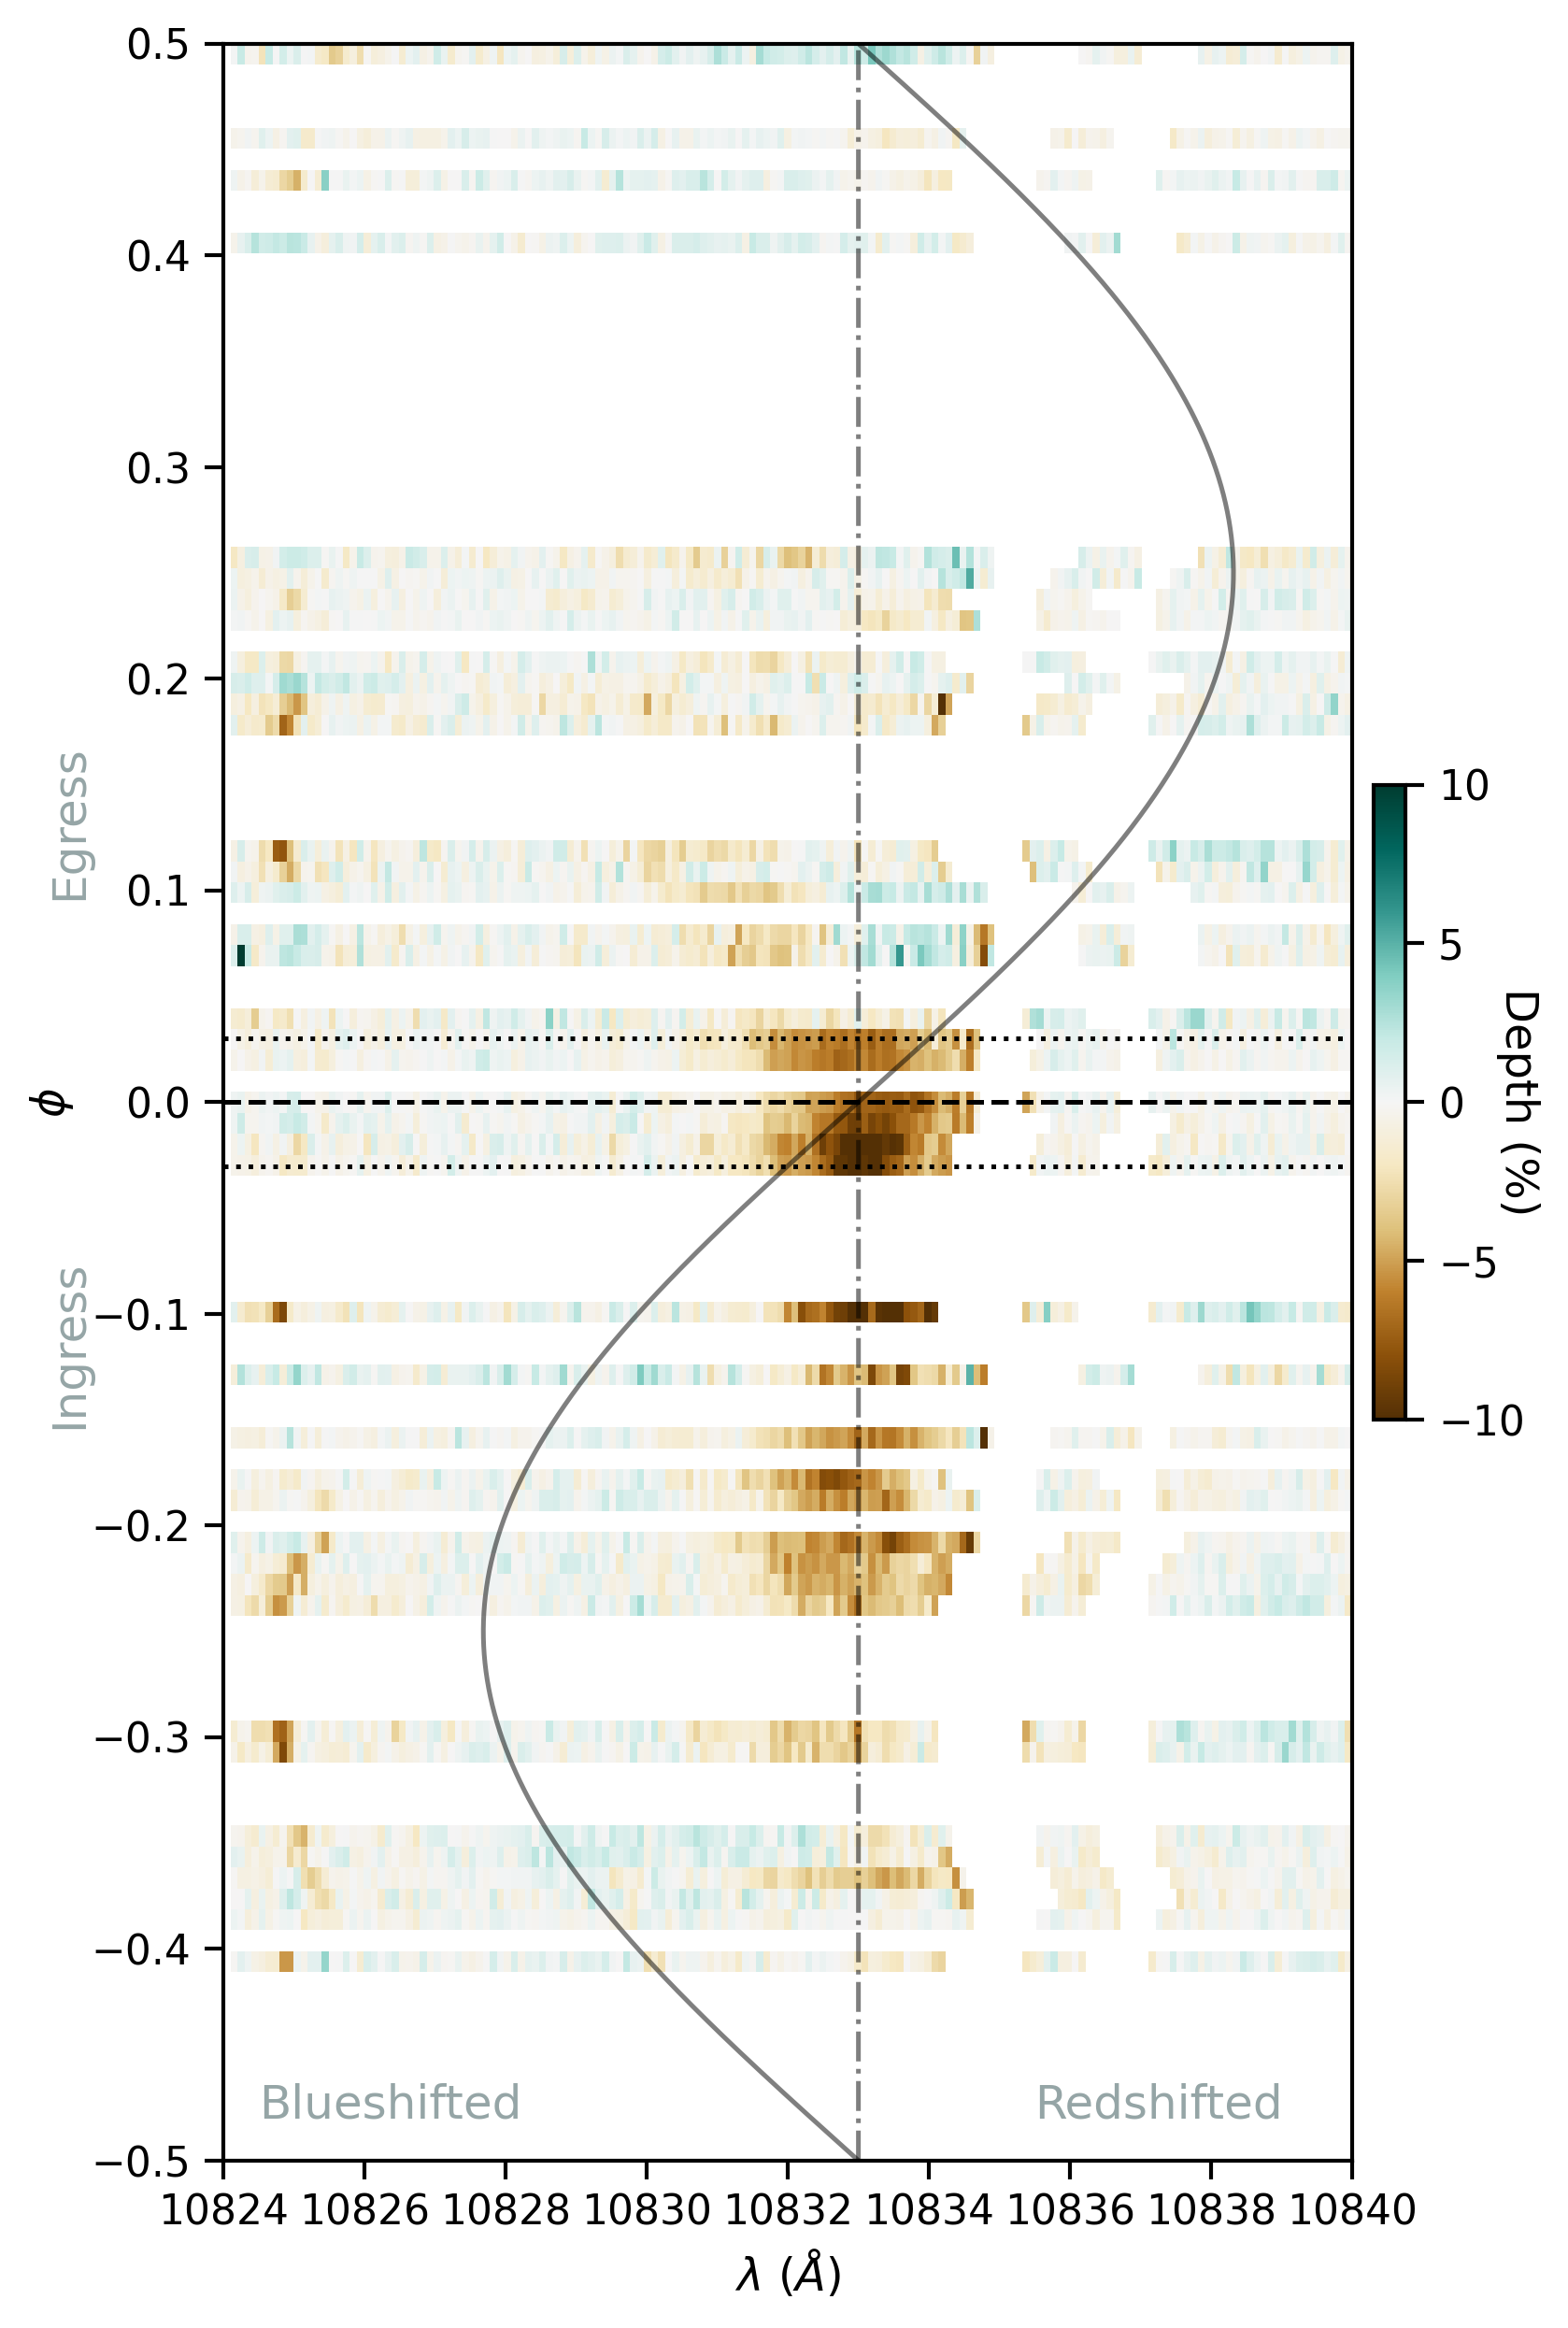
\includegraphics[width=\linewidth]{figures/phase_2D_diagram_resid.png}
    \caption{Absorption depth phase scan over the entire HAT-P-67b orbit from 41 visits with HPF.  }
    \label{fig:HPFscanResid}
\end{figure}


\begin{figure}
    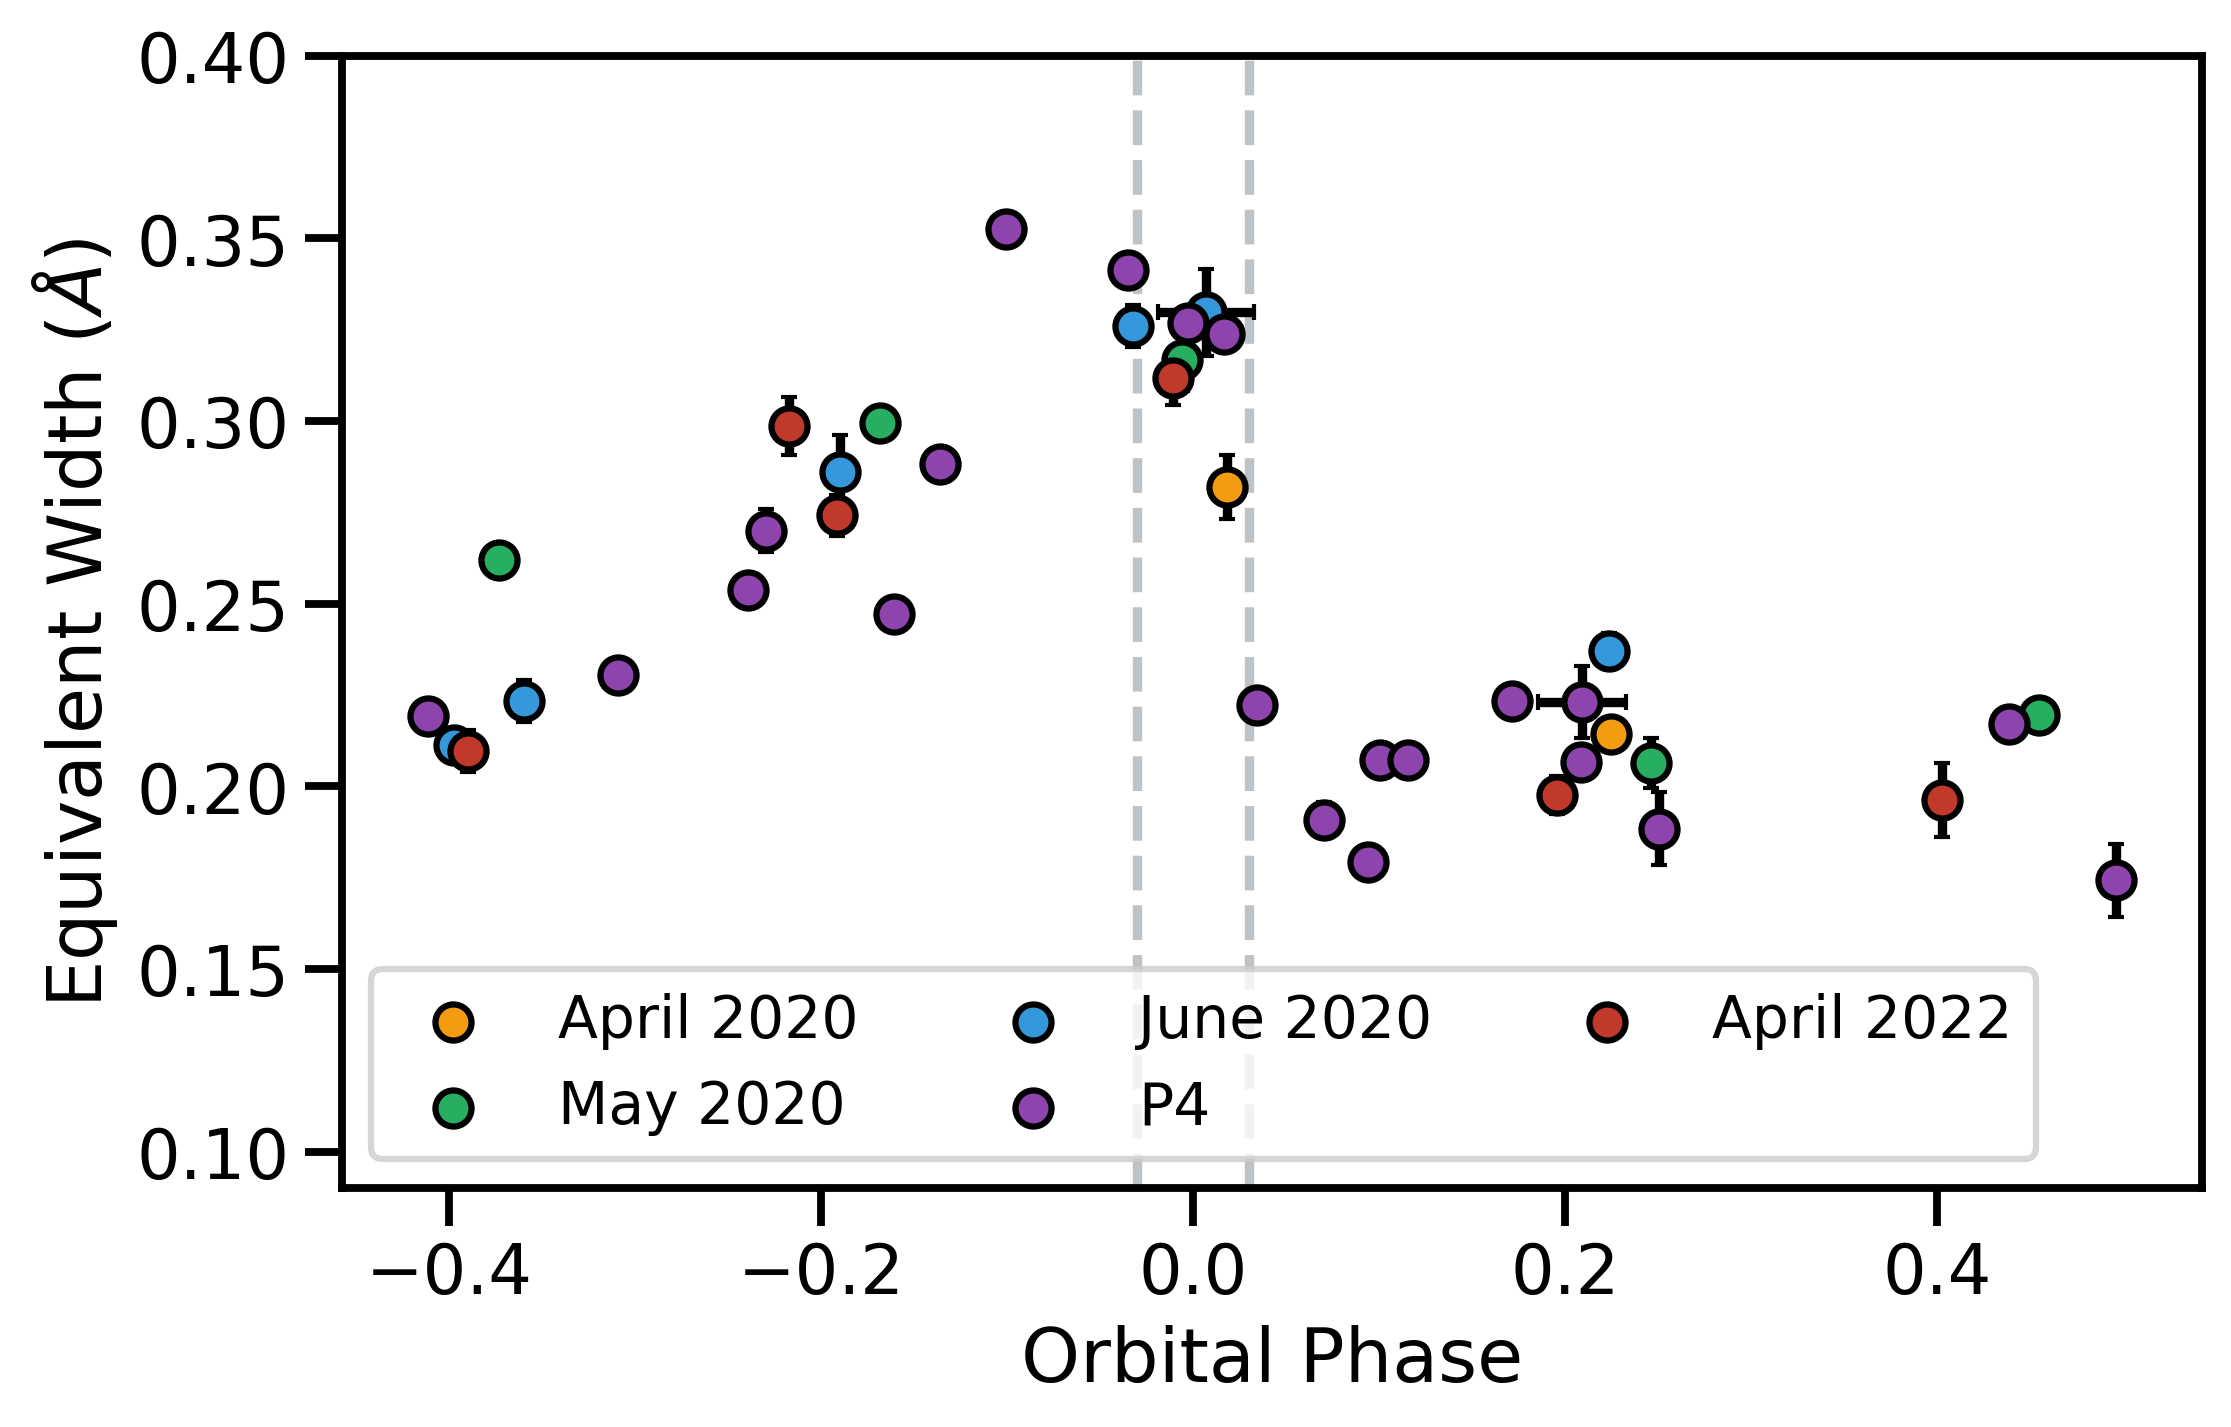
\includegraphics[width=\linewidth]{figures/HAT_P_67b_Helium10830EW_byCampaign.png}
    \caption{Time series EW lightcurve of Helium absorption in HAT-P-67b.  The system exhibits a characteristic absorption leading up to transit, followed by a sharp decline after transit passage.  }
    \label{fig:HPFtimeseries}
\end{figure}

\subsection{Calcium IR Triplet and other line diagnostics}
We examined the \ion{Ca}{2} IR Triplet lines (Ca IRT) for evidence of variability.  No variation was seen in these features, which were pre-processed in the same way as the Helium feature.  Figure \ref{fig:CaPhaseScan} shows a similar phase plot as Figure \ref{fig:HPFscanResid}, adapted to the line at 8662 \AA.  We see no conspicuous variability at this or any of the other Ca IRT lines.  We also found no detectable variability in the Pa$\delta$ line at 10050 \AA, nor other deep lines at 10330 \AA and elsewhere.  \ion{He}{1} 10833 appears to be the only conspicuously variable line in the HPF spectrum.

\begin{figure}
    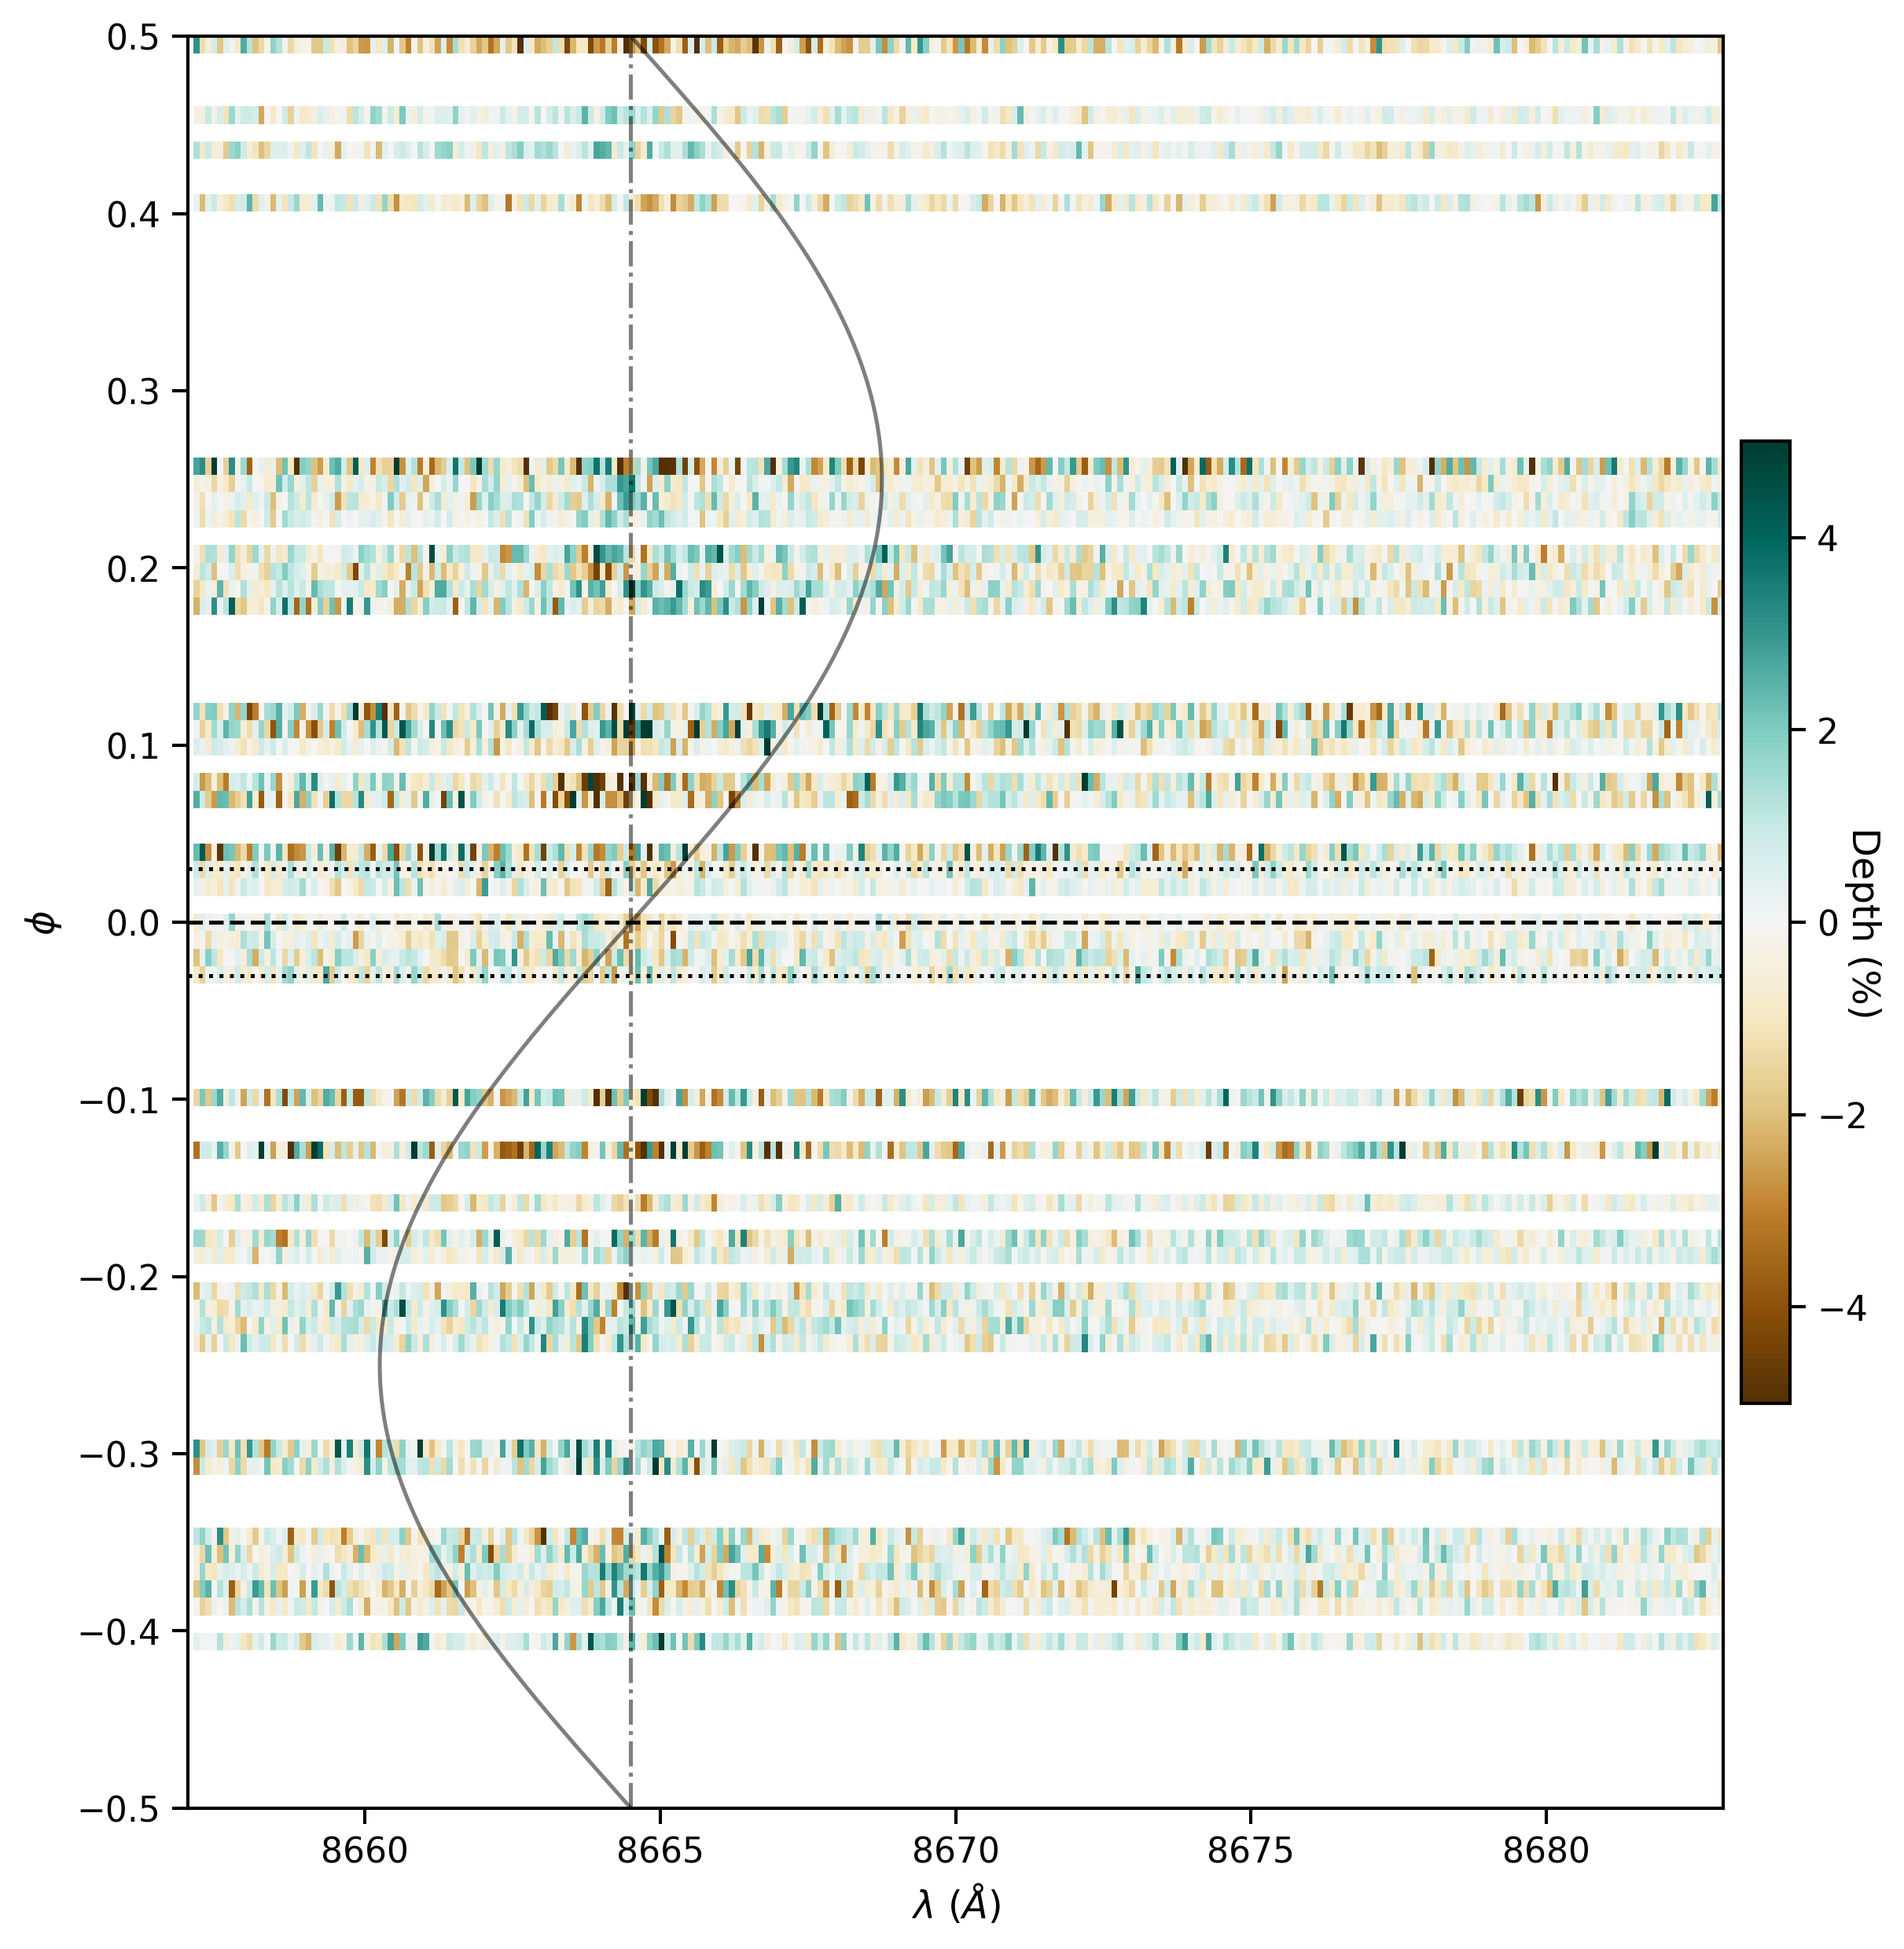
\includegraphics[width=\linewidth]{figures/Ca8662_phase_2D_diagram_resid.png}
    \caption{Non-detection of variability in the Calcium IR Triplet line at 8862 $\AA$.  No other HPF lines appear to show any variability.}
    \label{fig:CaPhaseScan}
\end{figure}

\subsection{Keck HIRES}
We retrieved 22 epochs of archival \emph{Keck HIRES} spectra via the Keck Observatory Archive (KOA). Of these, 19 were acquired through the iodine cell as reported by \citet{2017AJ....153..211Z}, providing RV orbit constraints.  The 14\arcsec~ slit height of the C2 decker appears to cause order overlap in \ion{Ca}{2} H and K lines, which contaminated the spectral extraction for 14 of the 22 spectra.  The 3\farcs5 B2 decker allowed the faithful extraction of this region for 6 spectra, which exhibit no perceptible \ion{Ca}{2} H and K variability.  The H~$\alpha$ region similarly exhibited no perceptible variability.  The timing of these spectra coincidentally missed the orbital phases ($-0.3$ to $+0.03$) where we see the greatest \ion{He}{1} 10833 \AA~ absorption excess, leaving open the possibility that detectable H~$\alpha$ absorption could be present at more favorable orbital phases.  New spectra or a more careful extraction of the archival C2 decker spectra would be needed.


\subsection{Velocity substructure}
Figure \ref{fig:HeliumScanZoom} shows a zoom-in of the in-transit portion of the absorption residual scan.  The scan appears to exhibit some velocity substructure.  At transit ingress, the absorption appears more centrally concentrated near the vertical 10833 \AA~ line.  The line depth gets slightly shallower with a slight redshift approaching transit midcenter.

\begin{figure}
    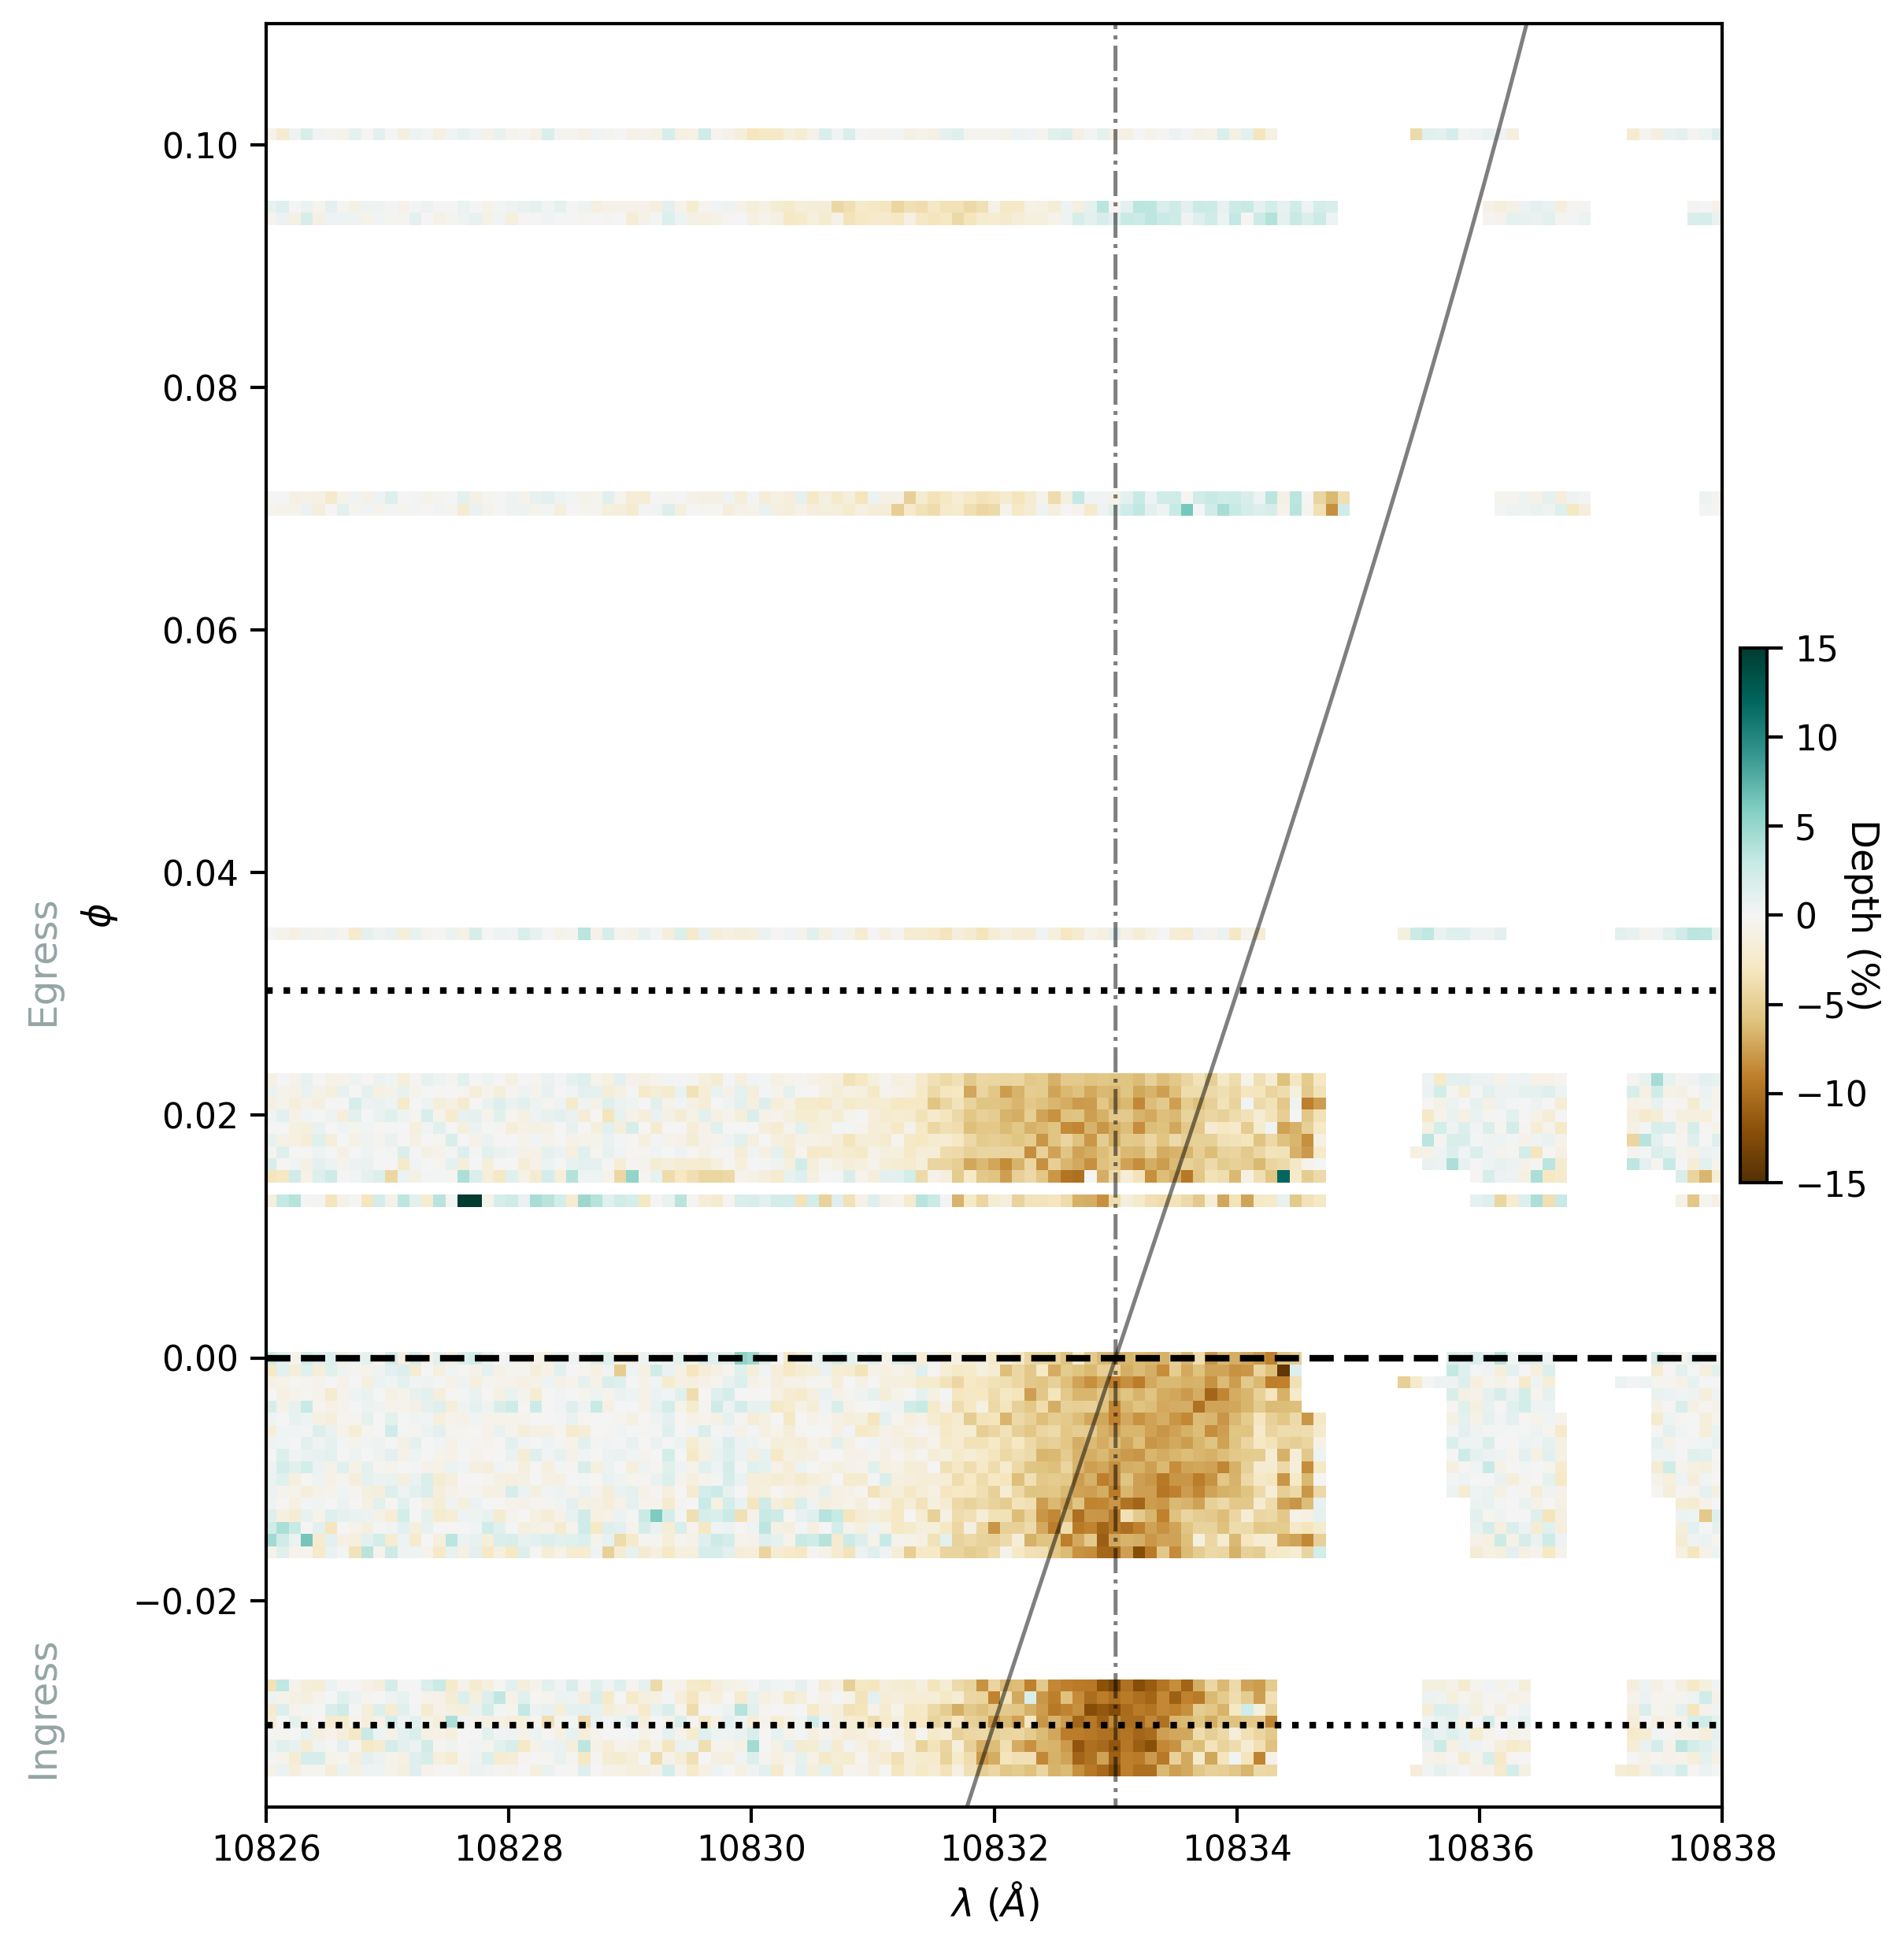
\includegraphics[width=\linewidth]{figures/phase_2D_diagram_zoom.png}
    \caption{A zoom-in of the in-transit and post-transit phase scan for the Helium 10830 triplet.  Some velocity substructure may be apparent.}
    \label{fig:HeliumScanZoom}
\end{figure}


\section{Atmospheric Escape}

\subsection{Size and geometry of outflow}
Helium absorption occurs predominantly before the planet is in-transit, indicating a \emph{leading} tail escaping the planet.  The excess occurs as early as 30\% of the orbital path.  That large fraction of an orbit translates to about 0.1 AU, 130 planetary radii, and well outside of the Roche Lobe, with its Hill radius of merely 2.6 planetary radii.  We are therefore primarily detecting gas that is entirely unbound from the planet.  The leading gas tail does not appear to accelerate, neither blue-shifting nor redshifting.   The bulk of the detectable unbound gas may therefore follow its own Keplerian trajectory at a slightly shorter period orbit, pulling away from the planet parallel to the orbital path.  Such a scenario may arise from preferential emission on the planet dayside, or other configurations that we discuss in Section \ref{secDiscuss}.

The out-of-transit excess exhibits approximately the same line width as the stellar lines, which are rotationally broadened by a $v\sin{i}$ of 30-35 km/s \citep{2017AJ....153..211Z}.  The large size of the gas stream overfills the transit chord, which means both the advancing blue side and receding red side of the rotating star are nearly continuously obscured in this spin-orbit-aligned system \citep{2017AJ....153..211Z}. The planet transits near the Stellar equator \citep{2017AJ....153..211Z}, meaning the transit chord covers about 10$\%$ of the projected stellar surface area.  Hypothetically a nearly 100$\%$ opaque optically thick stream of gas covering only the transit chord could reproduce the observed 10$\%$ absorption excess.  Alternatively---and more likely---an optically thin gas stream has some additional vertical extent perpendicular to the plane of orbit, which would act to overfill the entire projected stellar disk.  Assuming the gas has a spatially uniform optical depth of about 0.1 would reproduce the 10\% absorption excess.


\subsection{1D Parker wind models and mass loss rates}\label{pwinds}
The dramatic leading tail of atmospheric escape suggests that more complicated 3D hydrodymaic simulations coupled with stellar wind \citep{2022ApJ...926..226M} may be needed to depict the geometry faithfully.  Here we explore one-dimensional (1D) models, which offer ease of interpretation and rapid calculation.  We employ the open-source \texttt{p-winds} code \citep{2022A&A...659A..62D}, which implements a transonic 1D Parker wind model with radiative transfer of the Helium 10830 triplet \citep{2018ApJ...855L..11O,2020A&A...636A..13L}.

The predicted Helium ionization depends sensitively on the XUV flux \citep{2019ApJ...881..133O}.  Ideally we would have a measurement of the XUV spectrum of \hatp, but the limited facilities and distance of the source preclude these challenging observations.  Instead we constructed panchromatic X-ray to visible SEDs by scaling and stitching together synthetic spectra to provide a range of high and low $L_X/L_\mathrm{bol}$.  We chose a 6400 K PHOENIX \citep{husser13} solar metallicity photospheric spectral template with $\log{g}=3.5$, scaled to the solid angle seen by \hatpb.  The F7IV-V \object[tau Boo]{$\tau$ Boo} serves as the closest analog with synthetic x-ray coronal spectra available \citep{2011A&A...532A...6S}.  But \hatp resides closer to the Kraft break than does \object[tau Boo]{$\tau$ Boo}, and the move to hotter F stars may be associated with rapid changes in the stellar wind and other atmospheric changes leading to the prospect of much lower XUV luminosity for \hatp.  So there remains significant uncertainty about the applicability of the \object[tau Boo]{$\tau$ Boo} x-ray spectrum to \hatp.  We scaled the synthetic SED of \object[tau Boo]{$\tau$ Boo} retrieved from X-exoplanets \citep{2011A&A...532A...6S} so that the integral of ground-state ionizing photons ($\lambda<504\AA$) exhibited $L_X/L_\mathrm{bol} \in [10^{-7}, 10^{-5}]$.  Figure \ref{fig:XUV} shows two conceivable SEDs with a high and low radiation hardness.

\begin{figure}
    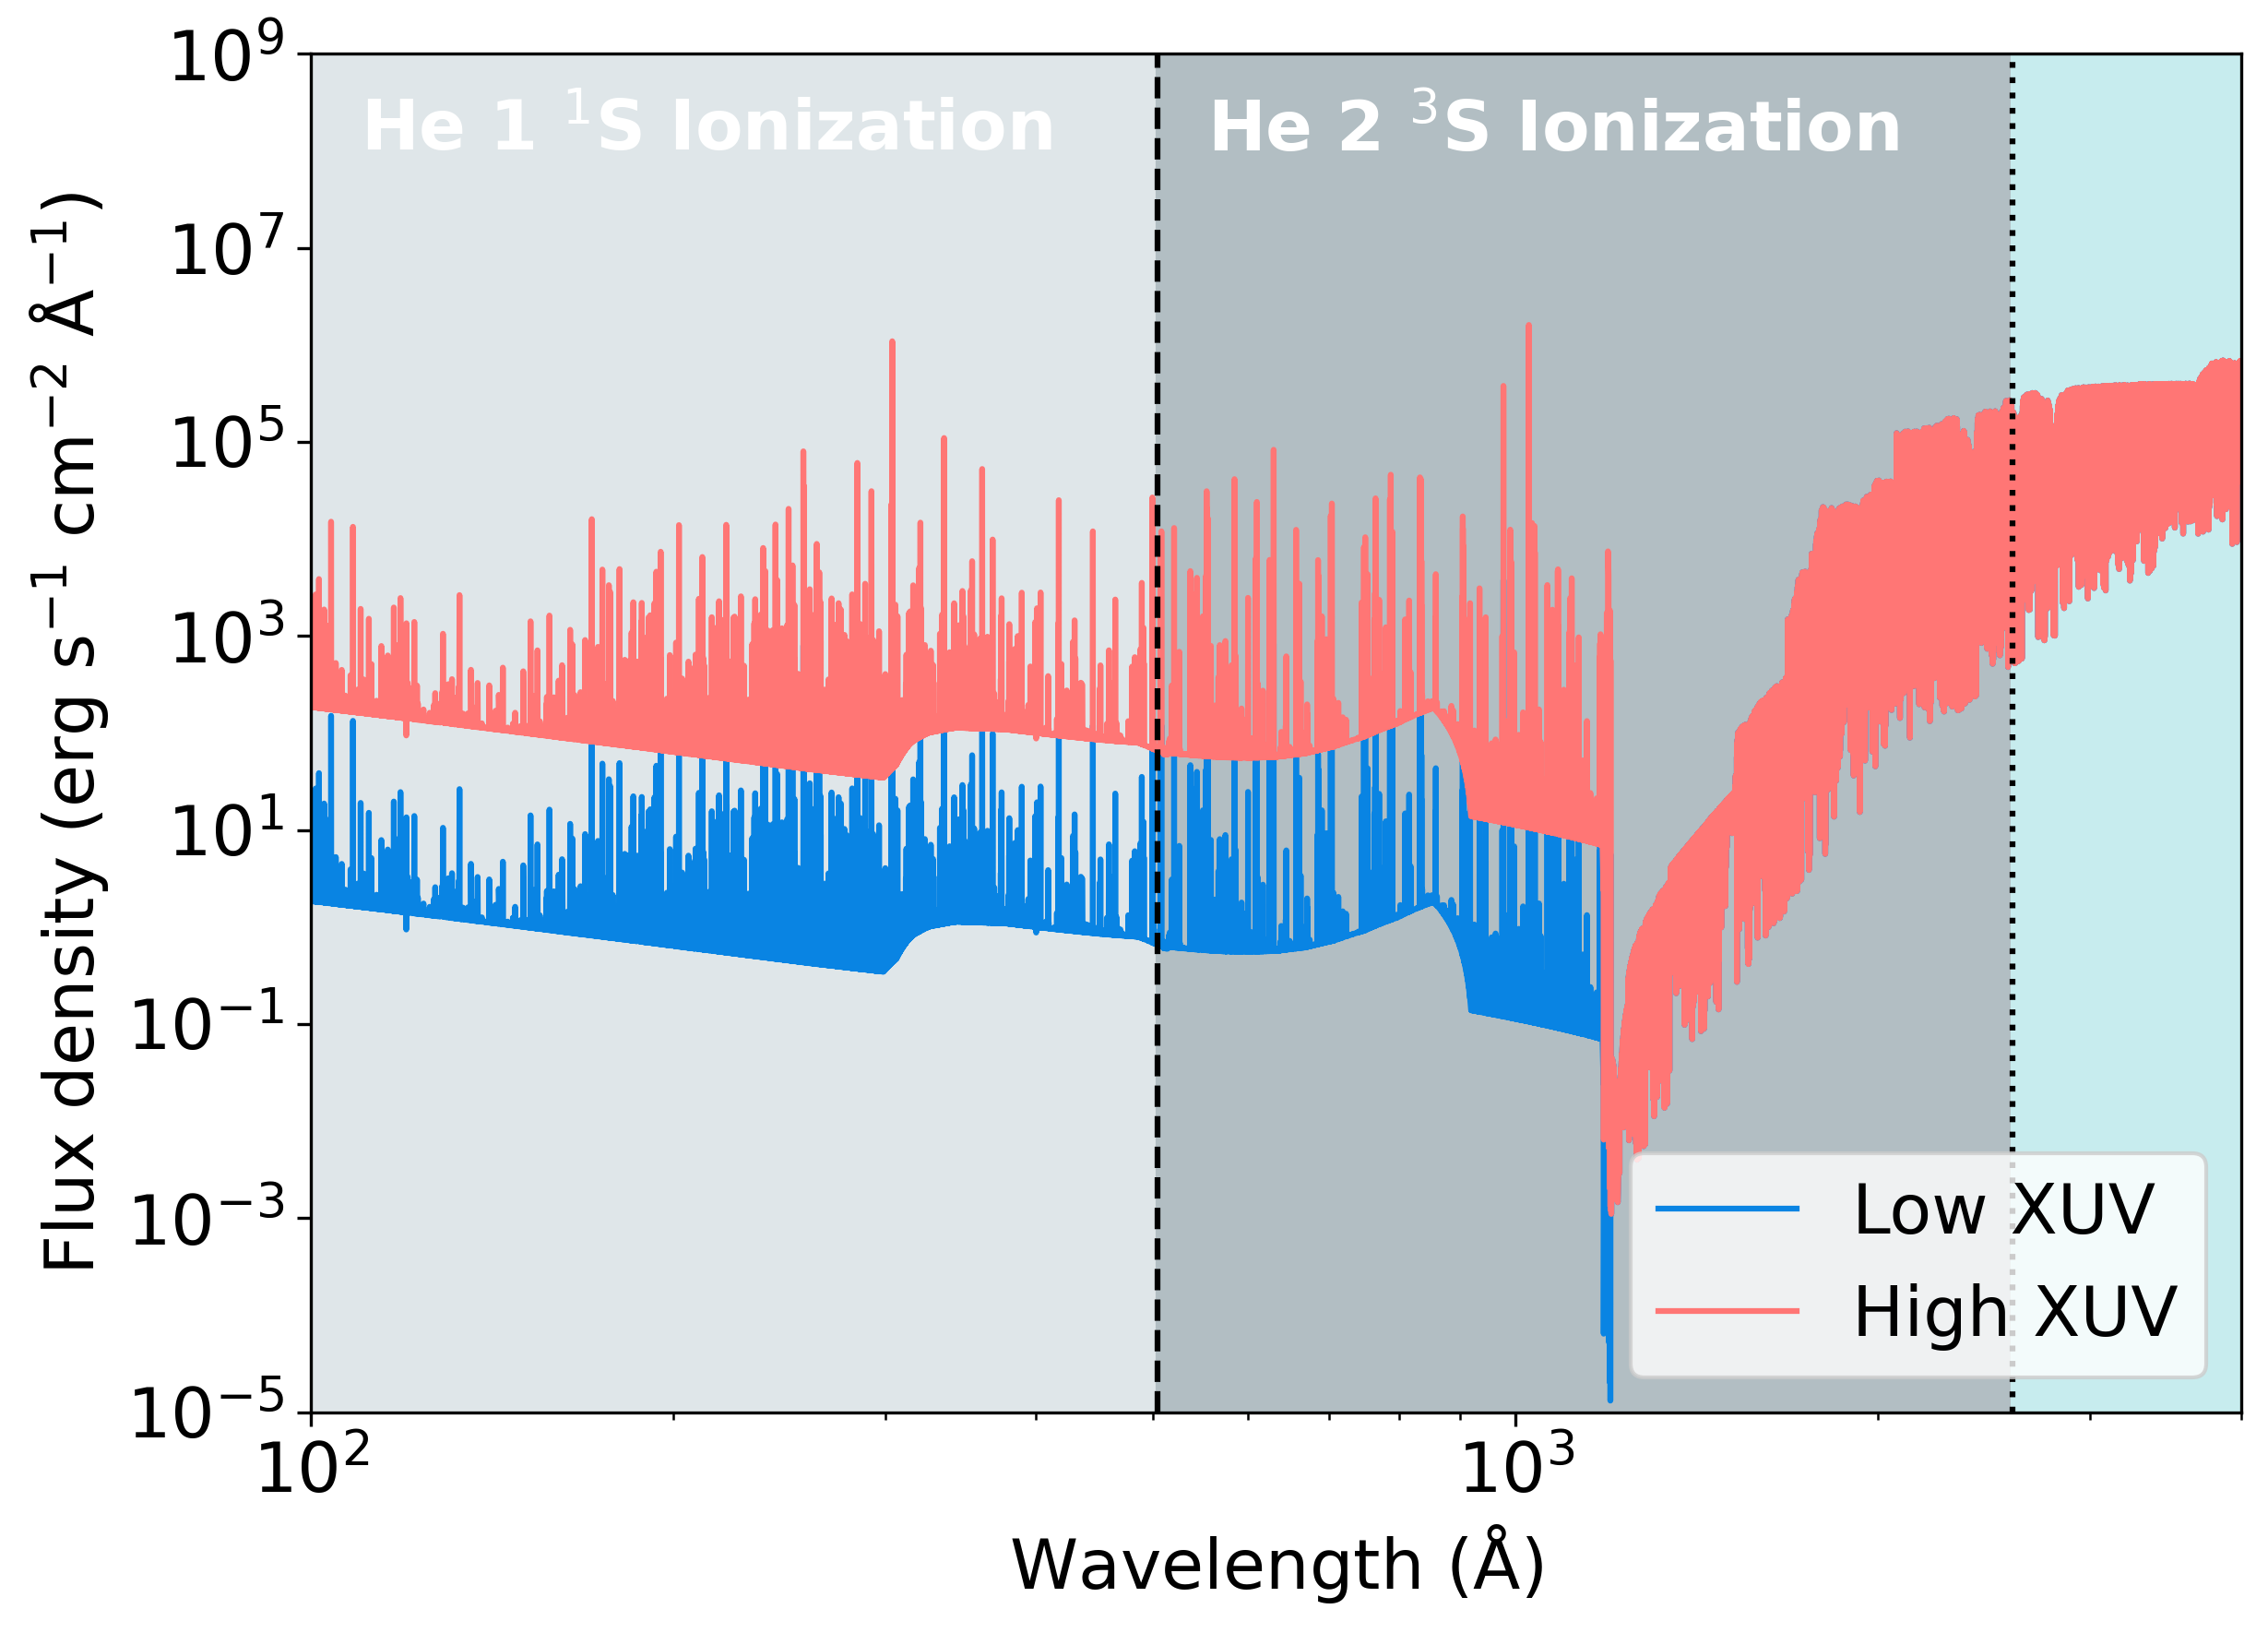
\includegraphics[width=\linewidth]{figures/XUV_flux_schematic.png}
    \caption{Synthetic XUV radiation scenarios for \hatpb.  }
    \label{fig:XUV}
\end{figure}

The SED shows two key features.   First the corona model does not extend all the way to 2600 $\AA$ photons capable of ionizing out of the 2 $^3$S Helium metastable state.  This apparent deficit probably does not matter because the F spectral type obtains most of its NUV photons ($\lambda\sim2600\AA$) from the Wein side of the photospheric spectrum, so the hardness of the radiation stems mostly from the assumptions of the corona flux level.  The wavelength-dependent cross section for absorption (not shown) is largest just blueward of the ionization thresholds, so the differences in the spectrum between 504 $\AA$ and 1000 $\AA$ have relatively little impact on the overall ionization out of the metastable state.

Equipped with these three SEDs of differing radiation hardness, we explored different mass loss rates and exosphere temperatures.  Figure \ref{fig:pwinds} shows one example model spectrum with $\dot{M} = 7\times10^{13}$ g/s, and $T_0=9100$~K, with the high XUV spectrum ($L_x/L_\mathrm{bol}=10^{-4}$).  The model spectrum exhibits approximately the same line width and depth as our HPF observations, making it a conceivable solution.

At least a few shortcomings limit the applicability of this 1D Parker wind model.  First, the model-dependent line profile (\emph{i.e. width and depth}) is degenerate with XUV flux, $\dot{M}$, and $T_0$, and so a range of these parameters can be fine-tuned to obtain a large range of mass loss rates consistent with the data and our limited understanding of the XUV flux.  Second, the 1D model breaks down when attempting to explain the inherently 3D leading tail geometry.  We discuss these two and other model-dependent interpretations in Section \ref{secDiscuss}.




\begin{figure}
    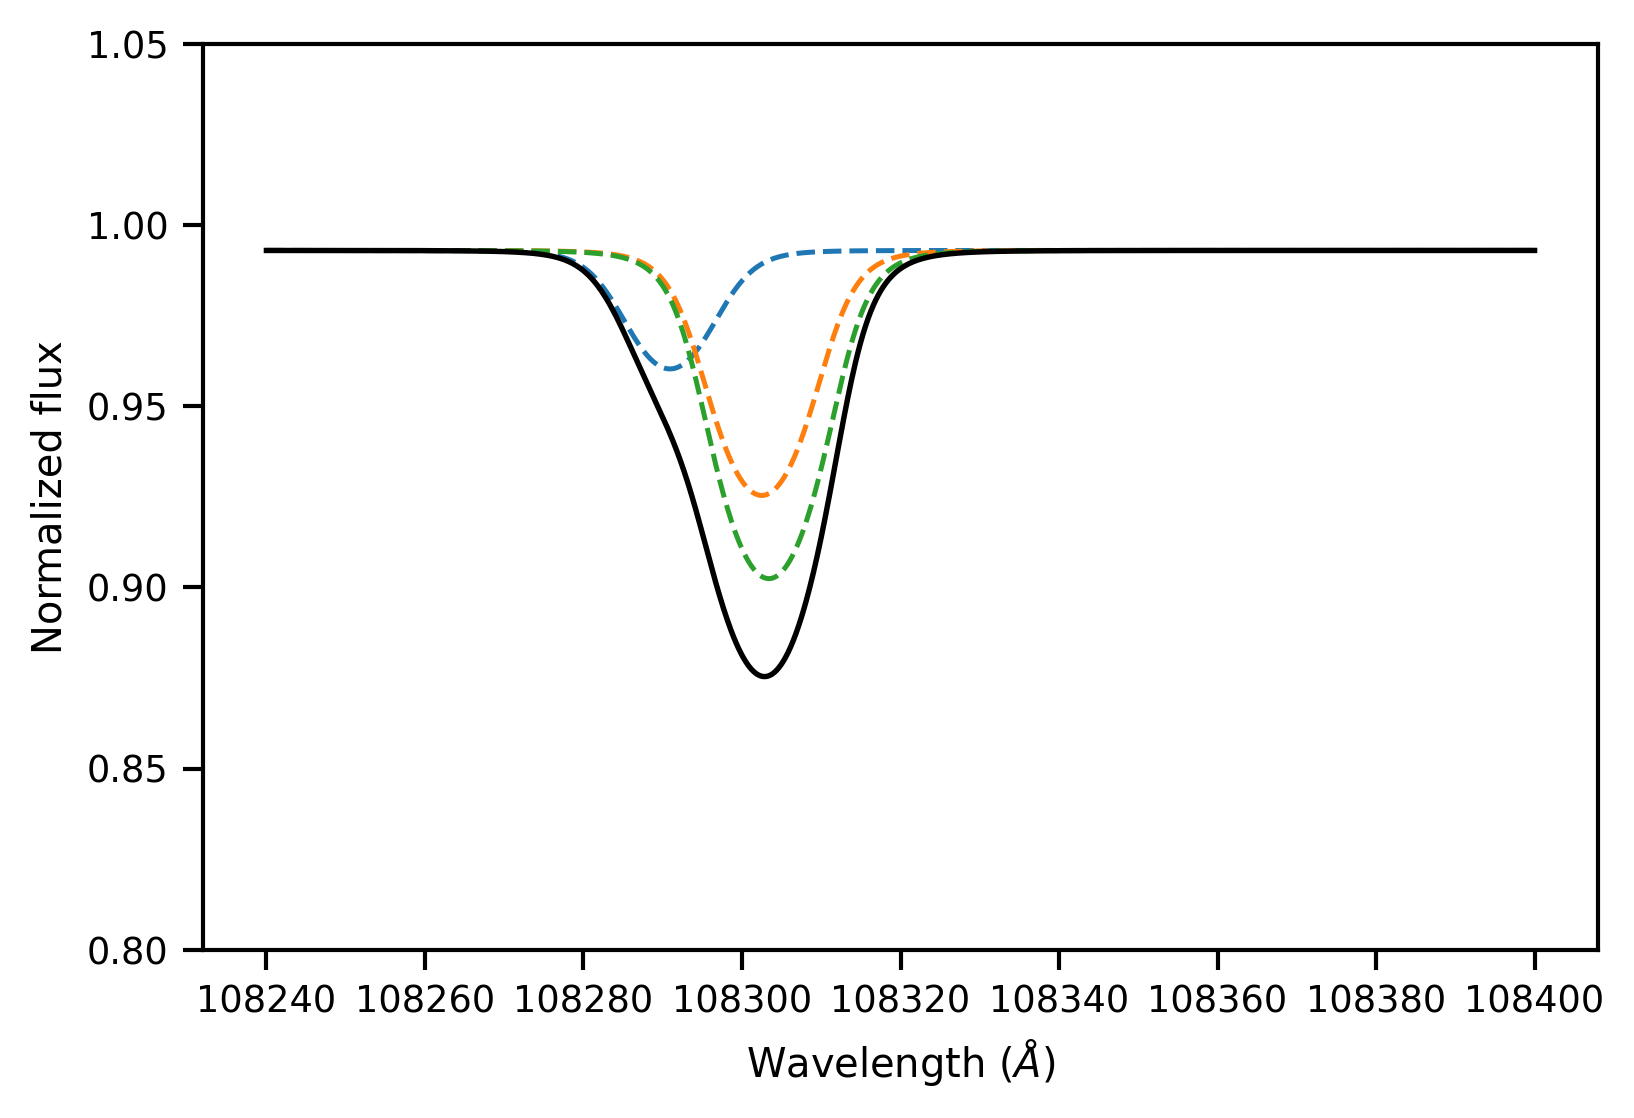
\includegraphics[width=\linewidth]{figures/pwinds_1D_higXUV_t1p2Gyr.png}
    \caption{Simulated 1D Parker wind model of Helium absorption in \hatpb.  The spectrum was generated with a mass loss rate of $1.7\times10^{13}$ g/s, exosphere gas temperature of 9100 K, and with the high XUV spectrum ($L_x/L_\mathrm{bol}=10^{-4}$) shown in Figure \ref{fig:XUV}.  The line depth and width broadly agrees with the width observed in HPF.}
    \label{fig:pwinds}
\end{figure}



\section{Discussion} \label{secDiscuss}

\subsection{Ohmic Dissipation and runaway escape}
\object{HAT-P-67 b} exhibits both dramatic atmospheric escape and significant radius inflation.  Ohmic dissipation stands out as a physical mechanism that could be responsible for both of these attributes.  \citet{2011ApJ...738....1B} showed that ohmic heating acts to inflate hot Jupiters, with low mass hot Jupiters overflowing their Roche lobes and leading to evaporation on Gyr timescales.  The Ohmic heating scenario requires only on a modest planetary magnetic field ($\sim$1 G) and enough photoionization to ionize some modest fraction of neutral metals.  The ``sweet spot'' for this phenomenon appears to prefer equilibrium temperatures in the range of $1500<T_\mathrm{eq}<2000$ K \citep{2011ApJ...738....1B}, well matched to HAT-P-67 b's $\sim$1900 K.  A plausible scaling law relationship approximate to an order-of-magnitude predicts an inflation timescales (Eq. 20 in \citet{2011ApJ...738....1B}):
\begin{equation}
    \tau_{\textit{infl}}\sim \left(\frac{0.01}{\epsilon} \right) \left(\frac{M}{M_{J}}\right)^2 \left(\frac{R_{J}}{R}\right)^3 \left(\frac{1500 \textrm{K}}{T_\mathrm{eff}}\right)^4 \textrm{Gyr}. \label{eqInflate}
\end{equation}


\noindent yielding an incredibly short 5 Myr timescale for \hatpb, assuming a typical $\epsilon\sim0.01$. The order of magnitude of this inflation timescale is so fleetingly short that \hatpb must be in the runaway stage of inflation, rapidly losing mass, and growing in surface area to fuel a positive feedback loop.


\subsection{Constraining mass loss rate}
A 5 Myr inflation timescale would imply an instantaneous $\dot{M}_\mathrm{infl}\sim10^{15}$ g/s, about 50 times larger than the 1D Parker wind model mass loss rate of $\dot{M}_\mathrm{1D}\sim2\times10^{13}$. Here we enumerate all of uncertainties that go into assessing mass loss rates to show that some in-between mass loss rate may be plausible.

First, the scaling law arguments that produced Equation \ref{eqInflate} (Eq. 20 of \citet{2011ApJ...738....1B}) were only proposed as order of magnitude estimates not to be taken too faithfully.  So a $10\times$ higher inflation timescale of 50 Myr would yield $\dot{M}_\mathrm{infl}\sim10^{14}$ g/s, still a very large mass loss rate, but only a factor of 5 away from the baseline 1D model.  Order unity uncertainties in the Ohmic dissipation efficiency $\epsilon$ may also contribute.

As mentioned in Section \ref{pwinds}, inferring the mass loss rate from observations is strongly model dependent, as seen in \censorbox{cite e.g. S.V. papers}.  The XUV flux, exosphere temperature $T_0$, and $\dot{M}$ are all at least partially degenerate.  In particular, the uncertain XUV-to-NUV flux ratio confounds the interpretation of the observed Helium signal.  Even the ``high XUV'' scenario in Figure \ref{fig:XUV} does not have enough ground-state ionizing photons to penetrate to within 5 $R_p$ of the planet surface.  This means that at best only 1 in $10^{6}$ Helium atoms participate in the observability of the Helium metastable triplet lines in the baseline 1D Parker wind model.  Turning down the XUV flux makes the signal even less observable.  A larger mass loss rate would be needed to explain the same observed HPF Helium absorption, if say only 1 in $10^{7}$ helium atoms are populating the metastable state.

Finally, the entire premise of the Parker wind model may be unjustified due to the inherently 3D geometry of the leading tail.  In the next section we critically examine the assumptions in the 1D Parker wind model.

\subsection{Causes for the leading tail}
Several physical phenomena could give rise to a leading tail geometry.  Here we explore two leading candidates: orbital shear and stellar wind confinement.

Figure \ref{fig:KeplerianShear} shows an illustration of Keplerian shear adapted to the system properties of \hatpb.  In this scenario, the wind launches primarily from the dayside, with relatively little or no wind launched from the nightside.  The wind initially launches radially from the planet, with the strongest wind located near the sub-stellar point, the line connecting the planet to star along the vertical axis in the figure.  Inefficient heating near the terminator subdues the mass loss in the $x-$direction, meaning that this wind exhibits not a hemi-spherical shape, more like a bulb or torpedo.  The gas increasingly experiences the star's Keplerian potential past the Roche lobe, accelerating in the direction of orbital motion, $+x$.  The accelerating column eventually overtakes the planet completely, with the prospect of extending to hundreds of planetary radii.

Stellar wind confinement...

\begin{figure}
    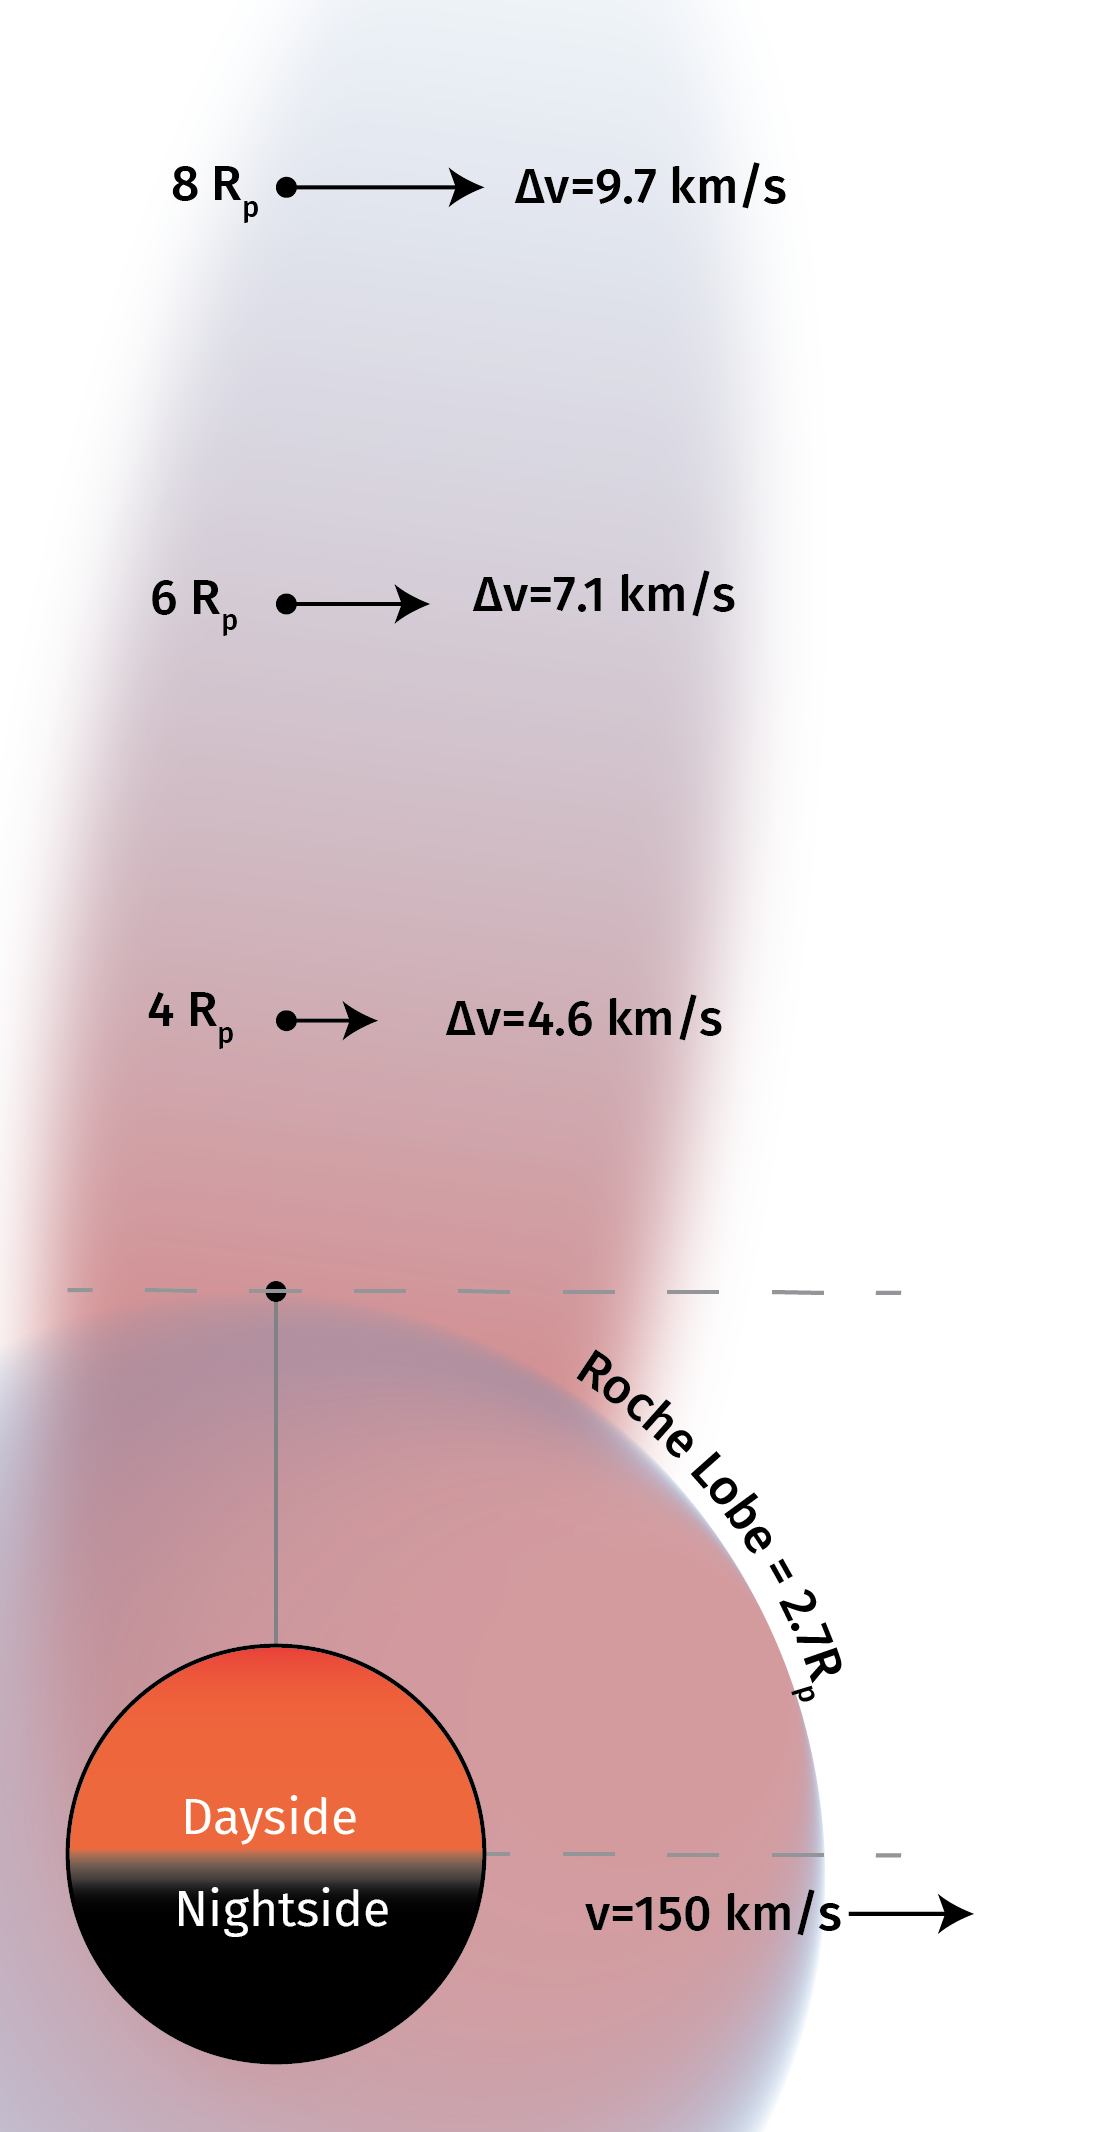
\includegraphics[width=0.8\linewidth]{figures/KeplerianShear_v0p3.png}
    \caption{Schematic of Keplerian orbital shear.  Locations outside the Roche lobe experience orbital shear from the Keplerian potential.  A wind launched primarily from the dayside will tend to form a leading tail.}
    \label{fig:KeplerianShear}
\end{figure}

\subsection{Critical examination of the Parker Wind model}

\begin{figure*}[t]
    \includegraphics[width=\linewidth]{figures/murray_clay_schematic_v0p2.png}
    \caption{Schematic of the relevant length scales in a stratified atmosphere, modeled after Figure 8 from \citet{2009ApJ...693...23M}.  The sonic point resides at a mere 2 atmospheric scale heights, and well below the photoionization level of Hydrogen, raising the possibility that the supersonic flow begins neutral and becomes ionized later on.}
    \label{fig:murrayClaySchematic}
\end{figure*}


An even more existential limit arises when we consider the assumptions of the isothermal Parker wind model, and the extreme geometry of \hatpb.  Figure \ref{fig:murrayClaySchematic} shows a schematic modeled after Figure 8 from \citet{2009ApJ...693...23M}.  The point at which the gas velocity exceeds the sound speed, the so-called sonic point, resides at 1.2 $R_p$, a mere $\sim9$ atmospheric scale heights from the planet surface.  The smallness of this radius can be understood from the significant effect of tidal gravity and the .  The pressure level here would be in the fractions of a millibar level, with an atmospheric temperature $\le T_\mathrm{eq}\sim10^3$~K and not yet the $T\sim10^4$~K exosphere range.  Depending on the mass loss rate, the transition from primarily neutral to primarily ionized plasma may occur outside or inside the sonic radius.


\subsection{Photoevaporation}
The prospect of Ohmic dissipation does not preclude the possibility that other mass loss drivers are at play.  Photoevaporation should simultaneously drive heating of the upper layers in the atmosphere, reinforcing the mass loss associated with Ohmic dissipation.  It is not clear which effect predominates.

\subsection{Cause for stellar modulation}
The \emph{TESS} lightcurve exhibits up to $0.36\%$ peak-to-valley modulation amplitude, with a characteristic timescale of $p=4.8-5.2$ days. Some sectors exhibit lower amplitudes.  The conventional interpretation would consign these cyclical modulations to the familiar stellar activity: surface features---either starspots, faculae, or plage---entering and exiting the projected stellar disk on the stellar rotation period comparable to the 4.8 day orbital period of planet b.  The cause for such orbital and rotational synchronization would then ostensibly be tides.  We examine the prospect of tides in the next subsection.

Alternatively, the exteme mass loss and credibility of the ohmic diffusion model motivates the prospect of Star Planet Magnetic Interaction (SPMI) that we consider now.  In this scenario, the magnetic field of the planet permeates the space between the star and planet.  Magnetic perturbations propagate via planetary magnetic fields with the Alfv\'en speed.  The planet can interact with the star if the Alfv\'en speed exceeds the stellar wind speed controling the bulk motion of intervening medium.  The magnetic field of the planet is not known, but the ohmic dissipation mechanism favors a limited range in the magnetic field strength: large enough to cause significant dissipative energy generation, but not too large to shut down charged particle motion entirely.  \citet{2011ApJ...738....1B} estimate this range as between about 1-30~G.

The non-detection of variability in the \ion{Ca}{2} H and K lines and H~$\alpha$ lines appears to disfavor this SPMI interpretation.

%\subsection{Timescale for tidal synchronization}


%\subsection{Hot Spot Scenario}
%The TESS 0.2\% flux variation could hypothetically arise from the foot-print of a star-planet interaction. Assuming that this increase in flux is due to a hot spot with a contrast of 200\% the ambient photosphere in the TESS bandpass, the hot spot would have a modest 5\% coverage fraction.  Thermal radiation from gravitational infall alone cannot explain the luminosity of this spot, so it would have to stem from a non-thermal cause.

%\subsection{Tidal Locking Calculation}
%The similarity of the rotation period with the orbital period suggests the star-planet system may be tidally locked.

%\subsection{Mass Loss Rate}
%A steady state mass loss rate greater than $2\times10^{12}$ g/s would erode the planet over the age of the stellar system.

%\subsection{Confinement to Stellar Wind}
%\subsection{Limits of Stellar Activity Metrics}
%\subsection{Comparison to Other Systems}
\section{Conclusions}


\clearpage
\pagebreak


\appendix
%\section{HPF spectra post-processing}
%\label{methods-details}


\begin{acknowledgements}

    This material is based upon work supported by the National Aeronautics and Space Administration under Grant Number 80NSSC20K0257 for the XRP program issued through the Science Mission Directorate.

    Based on observations obtained with the Hobby-Eberly Telescope (HET), which is a joint project of the University of Texas at Austin, the Pennsylvania State University, Ludwig-Maximillians-Universitaet Muenchen, and Georg-August Universitaet Goettingen. The HET is named in honor of its principal benefactors, William P. Hobby and Robert E. Eberly.

    These results are based on observations obtained with the Habitable-zone Planet Finder Spectrograph on the HET. The HPF team acknowledges support from NSF grants AST-1006676, AST-1126413, AST-1310885, AST-1517592, AST-1310875, ATI 2009889, ATI-2009982, AST-2108512, and the NASA Astrobiology Institute (NNA09DA76A) in the pursuit of precision radial velocities in the NIR. The HPF team also acknowledges support from the Heising-Simons Foundation via grant 2017-0494.

    This paper includes data collected with the TESS mission, obtained from the MAST data archive at the Space Telescope Science Institute (STScI). Funding for the TESS mission is provided by the NASA Explorer Program. STScI is operated by the Association of Universities for Research in Astronomy, Inc., under NASA contract NAS 5–26555.

    This research has made use of the Keck Observatory Archive (KOA), which is operated by the W. M. Keck Observatory and the NASA Exoplanet Science Institute (NExScI), under contract with the National Aeronautics and Space Administration.

    This research has made use of NASA's Astrophysics Data System.
\end{acknowledgements}

\facilities{HET (HPF), TESS, ASAS}

\software{  \texttt{pandas} \citep{mckinney10},
    \texttt{emcee} \citep{foreman13},
    \texttt{matplotlib} \citep{hunter07},
    \texttt{numpy} \citep{2020NumPy-Array},
    \texttt{scipy} \citep{2020SciPy-NMeth},
    \texttt{ipython} \citep{perez07},
    \texttt{seaborn} \citep{waskom14},
    \texttt{astropy} \citep{2022ApJ...935..167A},
    \texttt{muler} \citep{2022JOSS....7.4302G},
    \texttt{telfit} \citep{2014AJ....148...53G},
    \texttt{exoplanet} \citep{exoplanet:joss},
    \texttt{jupyter} \citep{Kluyver2016jupyter},
    \texttt{p-winds}, \citep{2022A&A...659A..62D}
}


\clearpage


\bibliography{ms}

\end{document}
